% Seminarul 5: Cozi groase și teoria valorilor extreme
% Statistica piețelor financiare -- Program de licență, Academia de Studii Economice din București
% GENERAT de latex/build_seminar5.py -- modificați generatorul, nu acest fișier.
% Implicit versiunea pentru studenți; versiunea profesorului este wrapper-ul *_solutions.tex.
\makeatletter\@ifundefined{ifsolutions}{\expandafter\newif\csname ifsolutions\endcsname}{}\makeatother

\newcommand{\coursename}{Statistica piețelor financiare}
\def\sfmlang{ro}
% Preambul comun SFM -- Statistica piețelor financiare / Statistics of Financial Markets (Beamer, 16:9)
% Același design ca MFM. Înainte de % Preambul comun SFM -- Statistica piețelor financiare / Statistics of Financial Markets (Beamer, 16:9)
% Același design ca MFM. Înainte de % Preambul comun SFM -- Statistica piețelor financiare / Statistics of Financial Markets (Beamer, 16:9)
% Același design ca MFM. Înainte de \input{../../latex/preamble} se definește
%   \newcommand{\coursename}{Statistics of Financial Markets}      (EN)
%   \newcommand{\coursename}{Statistica piețelor financiare}       (RO)  și  \def\sfmlang{ro}
% Fișierele .tex se află în EN/Courses, EN/Seminars, RO/Cursuri, RO/Seminarii (două niveluri sub rădăcină).
% Deck-urile sînt generate de latex/build_chapterN.py / build_seminarN.py (vezi latex/sfm_build.py).

\documentclass[9pt, aspectratio=169, t]{beamer}
\providecommand{\coursename}{Statistics of Financial Markets}

% Ensure content fits on slides
\setbeamersize{text margin left=8mm, text margin right=8mm}

%=============================================================================
% THEME AND STYLE CONFIGURATION
%=============================================================================
\usetheme{default}
% Using default theme for clean header/footer control

% Color Palette (matching Redispatch PDF)
\definecolor{MainBlue}{RGB}{26, 58, 110}
\definecolor{AccentBlue}{RGB}{26, 58, 110}
\definecolor{IDAred}{RGB}{205, 0, 0}
\definecolor{DarkGray}{RGB}{51, 51, 51}
\definecolor{MediumGray}{RGB}{128, 128, 128}
\definecolor{LightGray}{RGB}{248, 248, 248}
\definecolor{VeryLightGray}{RGB}{235, 235, 235}
\definecolor{KeynoteGray}{RGB}{218, 218, 218}
\definecolor{SectionGray}{RGB}{120, 120, 120}
\definecolor{FooterGray}{RGB}{100, 100, 100}
\definecolor{Crimson}{RGB}{220, 53, 69}
\definecolor{Forest}{RGB}{46, 125, 50}
\definecolor{Amber}{RGB}{181, 133, 63}
\definecolor{Orange}{RGB}{230, 126, 34}
\definecolor{Purple}{RGB}{142, 68, 173}

% Gradient background (exact Keynote 315° gradient: white to RGB 218,218,218)
\setbeamertemplate{background}{%
    \begin{tikzpicture}[remember picture, overlay]
        \shade[shading=axis, shading angle=315,
        top color=white, bottom color=KeynoteGray]
        (current page.south west) rectangle (current page.north east);
    \end{tikzpicture}%
}
% Fallback solid color for compatibility
\setbeamercolor{background canvas}{bg=}

\setbeamercolor{palette primary}{bg=MainBlue, fg=white}
\setbeamercolor{palette secondary}{bg=MainBlue!85, fg=white}
\setbeamercolor{palette tertiary}{bg=MainBlue!70, fg=white}
\setbeamercolor{structure}{fg=MainBlue}
\setbeamercolor{title}{fg=IDAred}
\setbeamercolor{frametitle}{fg=IDAred, bg=}
\setbeamercolor{block title}{bg=MainBlue, fg=white}
\setbeamercolor{block body}{bg=VeryLightGray, fg=DarkGray}
\setbeamercolor{block title alerted}{bg=Crimson, fg=white}
\setbeamercolor{block body alerted}{bg=Crimson!8, fg=DarkGray}
\setbeamercolor{block title example}{bg=Forest, fg=white}
\setbeamercolor{block body example}{bg=Forest!8, fg=DarkGray}
\setbeamercolor{item}{fg=MainBlue}

% Footer colors (override Madrid theme blue)
\setbeamercolor{author in head/foot}{fg=FooterGray, bg=}
\setbeamercolor{title in head/foot}{fg=FooterGray, bg=}
\setbeamercolor{date in head/foot}{fg=FooterGray, bg=}
\setbeamercolor{section in head/foot}{fg=FooterGray, bg=}
\setbeamercolor{subsection in head/foot}{fg=FooterGray, bg=}

% Bullet styles (apply everywhere including blocks)
\setbeamertemplate{itemize item}{\color{MainBlue}$\boxdot$}
\setbeamertemplate{itemize subitem}{\color{MainBlue}$\blacktriangleright$}
\setbeamertemplate{itemize subsubitem}{\color{MainBlue}\tiny$\bullet$}
\setbeamertemplate{itemize/enumerate body begin}{\normalsize}
\setbeamertemplate{itemize/enumerate subbody begin}{\normalsize}

% Item spacing - compact style
\setlength{\leftmargini}{10pt}       % Level 1: minimal indent
\setlength{\leftmarginii}{10pt}      % Level 2: minimal additional indent
% Compact list spacing (zero extra space before/after lists in blocks)
\makeatletter
\def\@listi{\leftmargin\leftmargini \topsep 0pt \parsep 0pt \itemsep 0pt}
\def\@listii{\leftmargin\leftmarginii \topsep 0pt \parsep 0pt \itemsep 0pt}
\makeatother

\setbeamertemplate{navigation symbols}{}

%=============================================================================
% CUSTOM HEADLINE
%=============================================================================
\setbeamertemplate{headline}{%
    \vskip10pt%
    \hbox to \paperwidth{%
        \hskip0.5cm%
        {\small\color{FooterGray}\renewcommand{\hyperlink}[2]{##2}\insertsectionhead}%
        \hfill%
        \textcolor{FooterGray}{\small\insertframenumber}%
        \hskip0.5cm%
    }%
    \vskip4pt%
    {\color{FooterGray}\hrule height 0.4pt}%
}

%=============================================================================
% CUSTOM FOOTER
%=============================================================================
\usepackage{fontawesome5}

\setbeamertemplate{footline}{%
    {\color{FooterGray}\hrule height 0.4pt}%
    \vskip4pt%
    \hbox to \paperwidth{%
        \hskip0.5cm%
        \textcolor{FooterGray}{\small\coursename}%
        \hfill%
        \raisebox{-0.1em}{%
            \begin{tikzpicture}[x=0.08em, y=0.08em, line width=0.4pt]
                \draw[FooterGray] (0,3) -- (1,4) -- (2,3.5) -- (3,5) -- (4,4) -- (5,6) -- (6,5.5) -- (7,4) -- (8,5) -- (9,7) -- (10,6) -- (11,5) -- (12,6.5) -- (13,8) -- (14,7) -- (15,6) -- (16,7.5) -- (17,9) -- (18,8) -- (19,7) -- (20,8.5) -- (21,10) -- (22,9) -- (23,8) -- (24,9.5);
            \end{tikzpicture}%
        }%
        \hskip0.5cm%
    }%
    \vskip6pt%
}

%=============================================================================
% PACKAGES
%=============================================================================
\usepackage[utf8]{inputenc}
\DeclareUnicodeCharacter{03B1}{\ensuremath{\alpha}}
\usepackage[T1]{fontenc}
\usepackage{amsmath, amssymb, amsthm}
\usepackage{mathtools}
\usepackage{bm}
\usepackage{tikz}
\usetikzlibrary{arrows.meta, positioning, shapes, calc, decorations.pathreplacing, shadings}
\usepackage{booktabs}
\usepackage{multirow}
\usepackage{array}
\usepackage{graphicx}
\usepackage{hyperref}
\usepackage{colortbl}
\usepackage{listings}
\lstset{language=Python, basicstyle=\ttfamily\scriptsize, keywordstyle=\color{MainBlue}\bfseries,
  commentstyle=\color{Forest}, stringstyle=\color{Crimson}, breaklines=true,
  frame=none, backgroundcolor=\color{VeryLightGray}, xleftmargin=2mm}
\hypersetup{colorlinks=true, linkcolor=MainBlue, urlcolor=MainBlue}
\graphicspath{{../../logos/}{../../charts/}{../../photos/}}
\usepackage{xcolor}
\hfuzz=2pt  % Suppress tiny overfull warnings (<2pt)
\vfuzz=2pt  % Suppress tiny vertical overfull warnings (<2pt)

%=============================================================================
% QUANTLET COMMANDS
%   \quantlet{<displayed name>}{<url>}       (generic, compatible with the older SFM decks)
%   \sfmquantlet{Ch_05}{SFM_ch5_garch}       -> https://github.com/danpele/SFM/tree/main/Quantlets/Ch_05/SFM_ch5_garch
%   \qlurl{<folder>} is defined per chapter by the generator (Quantlets/Ch_NN/<folder>)
%=============================================================================
\newcommand{\sfmrepo}{https://github.com/danpele/SFM}
\newcommand{\sfmqlbase}{https://github.com/danpele/SFM/tree/main/Quantlets}
\newcommand{\quantlet}[2]{%
    \hfill\href{#2}{%
        \raisebox{-0.15em}{
\includegraphics[height=0.7em]{ql_logo.png}}%
        \textcolor{MainBlue}{\tiny\ #1}%
    }%
}
\newcommand{\sfmquantlet}[2]{\quantlet{\detokenize{#2}}{\sfmqlbase/#1/#2}}

%=============================================================================
% NOTEBOOKS (Google Colab)
%   \colaburl{notebooks/EN/chapter5_seminar_notebook.ipynb} -> the Colab link of a file in the SFM repo
%   \nb: the chapter notebook (each seminar deck redefines it with \renewcommand)
%=============================================================================
\newcommand{\colaburl}[1]{https://colab.research.google.com/github/danpele/SFM/blob/main/#1}
\newcommand{\nb}{https://colab.research.google.com/github/danpele/SFM/tree/main/notebooks/EN}
\newcommand{\nbname}{notebooks/EN}

%=============================================================================
% SLIDE HELPERS (used by the generators; the same as in MFM)
%=============================================================================
% local font size for list bodies (the preamble forces \normalsize)
\newcommand{\itemsize}[1]{\setbeamertemplate{itemize/enumerate body begin}{#1}\setbeamertemplate{itemize/enumerate subbody begin}{#1}}
\newcommand{\intitle}[1]{{\hypersetup{urlcolor=white}#1}}   % white links inside coloured title bars
\newcommand{\imgcap}[1]{{\scriptsize #1}\\[0.5mm]}          % caption under a photo
\newcommand{\imgcredit}[2]{{\tiny\color{FooterGray}\href{#1}{#2}}}   % image credit: source URL, author/licence
\newcommand{\aiprompt}[1]{{\ttfamily\color{MainBlue}#1}}     % a prompt to an AI assistant

%=============================================================================
% SEMINARS: student version by default; the instructor wrapper *_solutions.tex sets \solutionstrue
%=============================================================================
\makeatletter\@ifundefined{ifsolutions}{\expandafter\newif\csname ifsolutions\endcsname}{}\makeatother
\newcommand{\solonly}[1]{\ifsolutions #1\fi}
\newcommand{\propsub}{\ifsolutions\else\framesubtitle{\ifdefined\sfmlang Rezolvarea se discută la seminar\else Solution discussed in class\fi}\fi}

%=============================================================================
% APPENDIX AND CHAPTER LINKS (latex/appendix_links.py writes the calls; it also re-declares these
% macros before \begin{document}, so the decks compile with or without this preamble block)
%=============================================================================
\providecommand{\sfmapplink}[3]{\hypertarget{#2}{}\hyperlink{#1}{\beamergotobutton{#3}}}
\providecommand{\sfmappback}[2]{\begin{tikzpicture}[remember picture,overlay]\node[anchor=south east] at ([xshift=-3mm,yshift=7mm]current page.south east){\hyperlink{#1}{\beamerreturnbutton{#2}}};\end{tikzpicture}}
\providecommand{\sfmchlink}[2]{\href{#1}{#2}}
\providecommand{\sfmchlinkt}[2]{\href{#1}{\usebeamercolor[fg]{frametitle}#2}}

%=============================================================================
% QUANTINAR COMMAND: link către un curs Quantinar (subiecte avansate)
%=============================================================================
\newcommand{\quantinar}[2]{%
    \href{#2}{%
        \raisebox{-0.15em}{
\includegraphics[height=0.8em]{qr_logo.png}}%
        \textcolor{MainBlue}{\scriptsize\ #1}%
    }%
}

%=============================================================================
% CUSTOM TITLE PAGE
%=============================================================================
\defbeamertemplate*{title page}{hybrid}[1][]
{
    \vspace{0.2cm}
    % Logos row - top header (with clickable links)
    \begin{center}
        \href{https://www.ase.ro}{
\includegraphics[height=1.0cm]{ase_logo.png}}\hspace{0.3cm}%
        \href{https://theida.net}{
\includegraphics[height=1.0cm]{ida_logo.png}}\hspace{0.3cm}%
        \href{https://blockchain-research-center.com}{
\includegraphics[height=1.0cm]{brc_logo.png}}\hspace{0.3cm}%
        \href{https://www.ai4efin.ase.ro}{
\includegraphics[height=1.0cm]{ai4efin_logo.png}}\hspace{0.3cm}%
        \href{https://ipe.ro/new}{
\includegraphics[height=1.0cm]{acad_logo.png}}\hspace{0.3cm}%
        \href{https://www.digital-finance-msca.com}{
\includegraphics[height=1.0cm]{msca_logo.png}}%
    \end{center}

    \vspace{0.6cm}

    % Main title with Q logos on sides (with clickable links)
    \begin{center}
        \begin{minipage}{0.1\textwidth}
            \centering
            \href{https://quantlet.com}{
\includegraphics[height=1.1cm]{ql_logo.png}}
        \end{minipage}%
        \begin{minipage}{0.78\textwidth}
            \centering
            {\LARGE\bfseries\usebeamercolor[fg]{title}\inserttitle}

            \vspace{0.3cm}

            {\usebeamerfont{subtitle}\usebeamercolor[fg]{title}\insertsubtitle}
        \end{minipage}%
        \begin{minipage}{0.1\textwidth}
            \centering
            \href{https://quantinar.com}{
\includegraphics[height=1.1cm]{qr_logo.png}}
        \end{minipage}
    \end{center}

    \vspace{0.6cm}

    % Authors (left aligned)
    \hspace{0.5cm}{\usebeamerfont{author}\insertauthor}

    \vspace{0.3cm}

    % Institute/Affiliations (left aligned)
    \hspace{0.5cm}\begin{minipage}[t]{0.9\textwidth}
        \raggedright\small\insertinstitute
    \end{minipage}
}

%=============================================================================
% THEOREM ENVIRONMENTS
%=============================================================================
\theoremstyle{definition}
\setbeamertemplate{theorems}[numbered]
\ifdefined\sfmlang
\newtheorem{defn}{Definiție}
\newtheorem{thm}{Teoremă}
\newtheorem{prop}{Propoziție}
\newtheorem{rmk}{Observație}
\else
\newtheorem{defn}{Definition}
\newtheorem{thm}{Theorem}
\newtheorem{prop}{Proposition}
\newtheorem{rmk}{Remark}
\fi

%=============================================================================
% CENTRED MINIPAGE (no extra vertical space)
%=============================================================================
\newenvironment{cminipage}[1]{%
    \par\noindent\hfill\begin{minipage}{#1}\ignorespaces
}{%
    \end{minipage}\hfill\null\par
}

%=============================================================================
% CUSTOM COMMANDS
%=============================================================================
\newcommand{\E}{\mathbb{E}}
\newcommand{\Var}{\text{Var}}
\newcommand{\Cov}{\text{Cov}}
\newcommand{\Corr}{\text{Corr}}
\newcommand{\R}{\mathbb{R}}
\newcommand{\N}{\mathbb{N}}
\newcommand{\Z}{\mathbb{Z}}
\newcommand{\B}{\mathbf{B}}
\newcommand{\imark}{\textcolor{MainBlue}{\textbullet}}
\newcommand{\RMSE}{\text{RMSE}}
\newcommand{\MAE}{\text{MAE}}
\newcommand{\MAPE}{\text{MAPE}}

 se definește
%   \newcommand{\coursename}{Statistics of Financial Markets}      (EN)
%   \newcommand{\coursename}{Statistica piețelor financiare}       (RO)  și  \def\sfmlang{ro}
% Fișierele .tex se află în EN/Courses, EN/Seminars, RO/Cursuri, RO/Seminarii (două niveluri sub rădăcină).
% Deck-urile sînt generate de latex/build_chapterN.py / build_seminarN.py (vezi latex/sfm_build.py).

\documentclass[9pt, aspectratio=169, t]{beamer}
\providecommand{\coursename}{Statistics of Financial Markets}

% Ensure content fits on slides
\setbeamersize{text margin left=8mm, text margin right=8mm}

%=============================================================================
% THEME AND STYLE CONFIGURATION
%=============================================================================
\usetheme{default}
% Using default theme for clean header/footer control

% Color Palette (matching Redispatch PDF)
\definecolor{MainBlue}{RGB}{26, 58, 110}
\definecolor{AccentBlue}{RGB}{26, 58, 110}
\definecolor{IDAred}{RGB}{205, 0, 0}
\definecolor{DarkGray}{RGB}{51, 51, 51}
\definecolor{MediumGray}{RGB}{128, 128, 128}
\definecolor{LightGray}{RGB}{248, 248, 248}
\definecolor{VeryLightGray}{RGB}{235, 235, 235}
\definecolor{KeynoteGray}{RGB}{218, 218, 218}
\definecolor{SectionGray}{RGB}{120, 120, 120}
\definecolor{FooterGray}{RGB}{100, 100, 100}
\definecolor{Crimson}{RGB}{220, 53, 69}
\definecolor{Forest}{RGB}{46, 125, 50}
\definecolor{Amber}{RGB}{181, 133, 63}
\definecolor{Orange}{RGB}{230, 126, 34}
\definecolor{Purple}{RGB}{142, 68, 173}

% Gradient background (exact Keynote 315° gradient: white to RGB 218,218,218)
\setbeamertemplate{background}{%
    \begin{tikzpicture}[remember picture, overlay]
        \shade[shading=axis, shading angle=315,
        top color=white, bottom color=KeynoteGray]
        (current page.south west) rectangle (current page.north east);
    \end{tikzpicture}%
}
% Fallback solid color for compatibility
\setbeamercolor{background canvas}{bg=}

\setbeamercolor{palette primary}{bg=MainBlue, fg=white}
\setbeamercolor{palette secondary}{bg=MainBlue!85, fg=white}
\setbeamercolor{palette tertiary}{bg=MainBlue!70, fg=white}
\setbeamercolor{structure}{fg=MainBlue}
\setbeamercolor{title}{fg=IDAred}
\setbeamercolor{frametitle}{fg=IDAred, bg=}
\setbeamercolor{block title}{bg=MainBlue, fg=white}
\setbeamercolor{block body}{bg=VeryLightGray, fg=DarkGray}
\setbeamercolor{block title alerted}{bg=Crimson, fg=white}
\setbeamercolor{block body alerted}{bg=Crimson!8, fg=DarkGray}
\setbeamercolor{block title example}{bg=Forest, fg=white}
\setbeamercolor{block body example}{bg=Forest!8, fg=DarkGray}
\setbeamercolor{item}{fg=MainBlue}

% Footer colors (override Madrid theme blue)
\setbeamercolor{author in head/foot}{fg=FooterGray, bg=}
\setbeamercolor{title in head/foot}{fg=FooterGray, bg=}
\setbeamercolor{date in head/foot}{fg=FooterGray, bg=}
\setbeamercolor{section in head/foot}{fg=FooterGray, bg=}
\setbeamercolor{subsection in head/foot}{fg=FooterGray, bg=}

% Bullet styles (apply everywhere including blocks)
\setbeamertemplate{itemize item}{\color{MainBlue}$\boxdot$}
\setbeamertemplate{itemize subitem}{\color{MainBlue}$\blacktriangleright$}
\setbeamertemplate{itemize subsubitem}{\color{MainBlue}\tiny$\bullet$}
\setbeamertemplate{itemize/enumerate body begin}{\normalsize}
\setbeamertemplate{itemize/enumerate subbody begin}{\normalsize}

% Item spacing - compact style
\setlength{\leftmargini}{10pt}       % Level 1: minimal indent
\setlength{\leftmarginii}{10pt}      % Level 2: minimal additional indent
% Compact list spacing (zero extra space before/after lists in blocks)
\makeatletter
\def\@listi{\leftmargin\leftmargini \topsep 0pt \parsep 0pt \itemsep 0pt}
\def\@listii{\leftmargin\leftmarginii \topsep 0pt \parsep 0pt \itemsep 0pt}
\makeatother

\setbeamertemplate{navigation symbols}{}

%=============================================================================
% CUSTOM HEADLINE
%=============================================================================
\setbeamertemplate{headline}{%
    \vskip10pt%
    \hbox to \paperwidth{%
        \hskip0.5cm%
        {\small\color{FooterGray}\renewcommand{\hyperlink}[2]{##2}\insertsectionhead}%
        \hfill%
        \textcolor{FooterGray}{\small\insertframenumber}%
        \hskip0.5cm%
    }%
    \vskip4pt%
    {\color{FooterGray}\hrule height 0.4pt}%
}

%=============================================================================
% CUSTOM FOOTER
%=============================================================================
\usepackage{fontawesome5}

\setbeamertemplate{footline}{%
    {\color{FooterGray}\hrule height 0.4pt}%
    \vskip4pt%
    \hbox to \paperwidth{%
        \hskip0.5cm%
        \textcolor{FooterGray}{\small\coursename}%
        \hfill%
        \raisebox{-0.1em}{%
            \begin{tikzpicture}[x=0.08em, y=0.08em, line width=0.4pt]
                \draw[FooterGray] (0,3) -- (1,4) -- (2,3.5) -- (3,5) -- (4,4) -- (5,6) -- (6,5.5) -- (7,4) -- (8,5) -- (9,7) -- (10,6) -- (11,5) -- (12,6.5) -- (13,8) -- (14,7) -- (15,6) -- (16,7.5) -- (17,9) -- (18,8) -- (19,7) -- (20,8.5) -- (21,10) -- (22,9) -- (23,8) -- (24,9.5);
            \end{tikzpicture}%
        }%
        \hskip0.5cm%
    }%
    \vskip6pt%
}

%=============================================================================
% PACKAGES
%=============================================================================
\usepackage[utf8]{inputenc}
\DeclareUnicodeCharacter{03B1}{\ensuremath{\alpha}}
\usepackage[T1]{fontenc}
\usepackage{amsmath, amssymb, amsthm}
\usepackage{mathtools}
\usepackage{bm}
\usepackage{tikz}
\usetikzlibrary{arrows.meta, positioning, shapes, calc, decorations.pathreplacing, shadings}
\usepackage{booktabs}
\usepackage{multirow}
\usepackage{array}
\usepackage{graphicx}
\usepackage{hyperref}
\usepackage{colortbl}
\usepackage{listings}
\lstset{language=Python, basicstyle=\ttfamily\scriptsize, keywordstyle=\color{MainBlue}\bfseries,
  commentstyle=\color{Forest}, stringstyle=\color{Crimson}, breaklines=true,
  frame=none, backgroundcolor=\color{VeryLightGray}, xleftmargin=2mm}
\hypersetup{colorlinks=true, linkcolor=MainBlue, urlcolor=MainBlue}
\graphicspath{{../../logos/}{../../charts/}{../../photos/}}
\usepackage{xcolor}
\hfuzz=2pt  % Suppress tiny overfull warnings (<2pt)
\vfuzz=2pt  % Suppress tiny vertical overfull warnings (<2pt)

%=============================================================================
% QUANTLET COMMANDS
%   \quantlet{<displayed name>}{<url>}       (generic, compatible with the older SFM decks)
%   \sfmquantlet{Ch_05}{SFM_ch5_garch}       -> https://github.com/danpele/SFM/tree/main/Quantlets/Ch_05/SFM_ch5_garch
%   \qlurl{<folder>} is defined per chapter by the generator (Quantlets/Ch_NN/<folder>)
%=============================================================================
\newcommand{\sfmrepo}{https://github.com/danpele/SFM}
\newcommand{\sfmqlbase}{https://github.com/danpele/SFM/tree/main/Quantlets}
\newcommand{\quantlet}[2]{%
    \hfill\href{#2}{%
        \raisebox{-0.15em}{
\includegraphics[height=0.7em]{ql_logo.png}}%
        \textcolor{MainBlue}{\tiny\ #1}%
    }%
}
\newcommand{\sfmquantlet}[2]{\quantlet{\detokenize{#2}}{\sfmqlbase/#1/#2}}

%=============================================================================
% NOTEBOOKS (Google Colab)
%   \colaburl{notebooks/EN/chapter5_seminar_notebook.ipynb} -> the Colab link of a file in the SFM repo
%   \nb: the chapter notebook (each seminar deck redefines it with \renewcommand)
%=============================================================================
\newcommand{\colaburl}[1]{https://colab.research.google.com/github/danpele/SFM/blob/main/#1}
\newcommand{\nb}{https://colab.research.google.com/github/danpele/SFM/tree/main/notebooks/EN}
\newcommand{\nbname}{notebooks/EN}

%=============================================================================
% SLIDE HELPERS (used by the generators; the same as in MFM)
%=============================================================================
% local font size for list bodies (the preamble forces \normalsize)
\newcommand{\itemsize}[1]{\setbeamertemplate{itemize/enumerate body begin}{#1}\setbeamertemplate{itemize/enumerate subbody begin}{#1}}
\newcommand{\intitle}[1]{{\hypersetup{urlcolor=white}#1}}   % white links inside coloured title bars
\newcommand{\imgcap}[1]{{\scriptsize #1}\\[0.5mm]}          % caption under a photo
\newcommand{\imgcredit}[2]{{\tiny\color{FooterGray}\href{#1}{#2}}}   % image credit: source URL, author/licence
\newcommand{\aiprompt}[1]{{\ttfamily\color{MainBlue}#1}}     % a prompt to an AI assistant

%=============================================================================
% SEMINARS: student version by default; the instructor wrapper *_solutions.tex sets \solutionstrue
%=============================================================================
\makeatletter\@ifundefined{ifsolutions}{\expandafter\newif\csname ifsolutions\endcsname}{}\makeatother
\newcommand{\solonly}[1]{\ifsolutions #1\fi}
\newcommand{\propsub}{\ifsolutions\else\framesubtitle{\ifdefined\sfmlang Rezolvarea se discută la seminar\else Solution discussed in class\fi}\fi}

%=============================================================================
% APPENDIX AND CHAPTER LINKS (latex/appendix_links.py writes the calls; it also re-declares these
% macros before \begin{document}, so the decks compile with or without this preamble block)
%=============================================================================
\providecommand{\sfmapplink}[3]{\hypertarget{#2}{}\hyperlink{#1}{\beamergotobutton{#3}}}
\providecommand{\sfmappback}[2]{\begin{tikzpicture}[remember picture,overlay]\node[anchor=south east] at ([xshift=-3mm,yshift=7mm]current page.south east){\hyperlink{#1}{\beamerreturnbutton{#2}}};\end{tikzpicture}}
\providecommand{\sfmchlink}[2]{\href{#1}{#2}}
\providecommand{\sfmchlinkt}[2]{\href{#1}{\usebeamercolor[fg]{frametitle}#2}}

%=============================================================================
% QUANTINAR COMMAND: link către un curs Quantinar (subiecte avansate)
%=============================================================================
\newcommand{\quantinar}[2]{%
    \href{#2}{%
        \raisebox{-0.15em}{
\includegraphics[height=0.8em]{qr_logo.png}}%
        \textcolor{MainBlue}{\scriptsize\ #1}%
    }%
}

%=============================================================================
% CUSTOM TITLE PAGE
%=============================================================================
\defbeamertemplate*{title page}{hybrid}[1][]
{
    \vspace{0.2cm}
    % Logos row - top header (with clickable links)
    \begin{center}
        \href{https://www.ase.ro}{
\includegraphics[height=1.0cm]{ase_logo.png}}\hspace{0.3cm}%
        \href{https://theida.net}{
\includegraphics[height=1.0cm]{ida_logo.png}}\hspace{0.3cm}%
        \href{https://blockchain-research-center.com}{
\includegraphics[height=1.0cm]{brc_logo.png}}\hspace{0.3cm}%
        \href{https://www.ai4efin.ase.ro}{
\includegraphics[height=1.0cm]{ai4efin_logo.png}}\hspace{0.3cm}%
        \href{https://ipe.ro/new}{
\includegraphics[height=1.0cm]{acad_logo.png}}\hspace{0.3cm}%
        \href{https://www.digital-finance-msca.com}{
\includegraphics[height=1.0cm]{msca_logo.png}}%
    \end{center}

    \vspace{0.6cm}

    % Main title with Q logos on sides (with clickable links)
    \begin{center}
        \begin{minipage}{0.1\textwidth}
            \centering
            \href{https://quantlet.com}{
\includegraphics[height=1.1cm]{ql_logo.png}}
        \end{minipage}%
        \begin{minipage}{0.78\textwidth}
            \centering
            {\LARGE\bfseries\usebeamercolor[fg]{title}\inserttitle}

            \vspace{0.3cm}

            {\usebeamerfont{subtitle}\usebeamercolor[fg]{title}\insertsubtitle}
        \end{minipage}%
        \begin{minipage}{0.1\textwidth}
            \centering
            \href{https://quantinar.com}{
\includegraphics[height=1.1cm]{qr_logo.png}}
        \end{minipage}
    \end{center}

    \vspace{0.6cm}

    % Authors (left aligned)
    \hspace{0.5cm}{\usebeamerfont{author}\insertauthor}

    \vspace{0.3cm}

    % Institute/Affiliations (left aligned)
    \hspace{0.5cm}\begin{minipage}[t]{0.9\textwidth}
        \raggedright\small\insertinstitute
    \end{minipage}
}

%=============================================================================
% THEOREM ENVIRONMENTS
%=============================================================================
\theoremstyle{definition}
\setbeamertemplate{theorems}[numbered]
\ifdefined\sfmlang
\newtheorem{defn}{Definiție}
\newtheorem{thm}{Teoremă}
\newtheorem{prop}{Propoziție}
\newtheorem{rmk}{Observație}
\else
\newtheorem{defn}{Definition}
\newtheorem{thm}{Theorem}
\newtheorem{prop}{Proposition}
\newtheorem{rmk}{Remark}
\fi

%=============================================================================
% CENTRED MINIPAGE (no extra vertical space)
%=============================================================================
\newenvironment{cminipage}[1]{%
    \par\noindent\hfill\begin{minipage}{#1}\ignorespaces
}{%
    \end{minipage}\hfill\null\par
}

%=============================================================================
% CUSTOM COMMANDS
%=============================================================================
\newcommand{\E}{\mathbb{E}}
\newcommand{\Var}{\text{Var}}
\newcommand{\Cov}{\text{Cov}}
\newcommand{\Corr}{\text{Corr}}
\newcommand{\R}{\mathbb{R}}
\newcommand{\N}{\mathbb{N}}
\newcommand{\Z}{\mathbb{Z}}
\newcommand{\B}{\mathbf{B}}
\newcommand{\imark}{\textcolor{MainBlue}{\textbullet}}
\newcommand{\RMSE}{\text{RMSE}}
\newcommand{\MAE}{\text{MAE}}
\newcommand{\MAPE}{\text{MAPE}}

 se definește
%   \newcommand{\coursename}{Statistics of Financial Markets}      (EN)
%   \newcommand{\coursename}{Statistica piețelor financiare}       (RO)  și  \def\sfmlang{ro}
% Fișierele .tex se află în EN/Courses, EN/Seminars, RO/Cursuri, RO/Seminarii (două niveluri sub rădăcină).
% Deck-urile sînt generate de latex/build_chapterN.py / build_seminarN.py (vezi latex/sfm_build.py).

\documentclass[9pt, aspectratio=169, t]{beamer}
\providecommand{\coursename}{Statistics of Financial Markets}

% Ensure content fits on slides
\setbeamersize{text margin left=8mm, text margin right=8mm}

%=============================================================================
% THEME AND STYLE CONFIGURATION
%=============================================================================
\usetheme{default}
% Using default theme for clean header/footer control

% Color Palette (matching Redispatch PDF)
\definecolor{MainBlue}{RGB}{26, 58, 110}
\definecolor{AccentBlue}{RGB}{26, 58, 110}
\definecolor{IDAred}{RGB}{205, 0, 0}
\definecolor{DarkGray}{RGB}{51, 51, 51}
\definecolor{MediumGray}{RGB}{128, 128, 128}
\definecolor{LightGray}{RGB}{248, 248, 248}
\definecolor{VeryLightGray}{RGB}{235, 235, 235}
\definecolor{KeynoteGray}{RGB}{218, 218, 218}
\definecolor{SectionGray}{RGB}{120, 120, 120}
\definecolor{FooterGray}{RGB}{100, 100, 100}
\definecolor{Crimson}{RGB}{220, 53, 69}
\definecolor{Forest}{RGB}{46, 125, 50}
\definecolor{Amber}{RGB}{181, 133, 63}
\definecolor{Orange}{RGB}{230, 126, 34}
\definecolor{Purple}{RGB}{142, 68, 173}

% Gradient background (exact Keynote 315° gradient: white to RGB 218,218,218)
\setbeamertemplate{background}{%
    \begin{tikzpicture}[remember picture, overlay]
        \shade[shading=axis, shading angle=315,
        top color=white, bottom color=KeynoteGray]
        (current page.south west) rectangle (current page.north east);
    \end{tikzpicture}%
}
% Fallback solid color for compatibility
\setbeamercolor{background canvas}{bg=}

\setbeamercolor{palette primary}{bg=MainBlue, fg=white}
\setbeamercolor{palette secondary}{bg=MainBlue!85, fg=white}
\setbeamercolor{palette tertiary}{bg=MainBlue!70, fg=white}
\setbeamercolor{structure}{fg=MainBlue}
\setbeamercolor{title}{fg=IDAred}
\setbeamercolor{frametitle}{fg=IDAred, bg=}
\setbeamercolor{block title}{bg=MainBlue, fg=white}
\setbeamercolor{block body}{bg=VeryLightGray, fg=DarkGray}
\setbeamercolor{block title alerted}{bg=Crimson, fg=white}
\setbeamercolor{block body alerted}{bg=Crimson!8, fg=DarkGray}
\setbeamercolor{block title example}{bg=Forest, fg=white}
\setbeamercolor{block body example}{bg=Forest!8, fg=DarkGray}
\setbeamercolor{item}{fg=MainBlue}

% Footer colors (override Madrid theme blue)
\setbeamercolor{author in head/foot}{fg=FooterGray, bg=}
\setbeamercolor{title in head/foot}{fg=FooterGray, bg=}
\setbeamercolor{date in head/foot}{fg=FooterGray, bg=}
\setbeamercolor{section in head/foot}{fg=FooterGray, bg=}
\setbeamercolor{subsection in head/foot}{fg=FooterGray, bg=}

% Bullet styles (apply everywhere including blocks)
\setbeamertemplate{itemize item}{\color{MainBlue}$\boxdot$}
\setbeamertemplate{itemize subitem}{\color{MainBlue}$\blacktriangleright$}
\setbeamertemplate{itemize subsubitem}{\color{MainBlue}\tiny$\bullet$}
\setbeamertemplate{itemize/enumerate body begin}{\normalsize}
\setbeamertemplate{itemize/enumerate subbody begin}{\normalsize}

% Item spacing - compact style
\setlength{\leftmargini}{10pt}       % Level 1: minimal indent
\setlength{\leftmarginii}{10pt}      % Level 2: minimal additional indent
% Compact list spacing (zero extra space before/after lists in blocks)
\makeatletter
\def\@listi{\leftmargin\leftmargini \topsep 0pt \parsep 0pt \itemsep 0pt}
\def\@listii{\leftmargin\leftmarginii \topsep 0pt \parsep 0pt \itemsep 0pt}
\makeatother

\setbeamertemplate{navigation symbols}{}

%=============================================================================
% CUSTOM HEADLINE
%=============================================================================
\setbeamertemplate{headline}{%
    \vskip10pt%
    \hbox to \paperwidth{%
        \hskip0.5cm%
        {\small\color{FooterGray}\renewcommand{\hyperlink}[2]{##2}\insertsectionhead}%
        \hfill%
        \textcolor{FooterGray}{\small\insertframenumber}%
        \hskip0.5cm%
    }%
    \vskip4pt%
    {\color{FooterGray}\hrule height 0.4pt}%
}

%=============================================================================
% CUSTOM FOOTER
%=============================================================================
\usepackage{fontawesome5}

\setbeamertemplate{footline}{%
    {\color{FooterGray}\hrule height 0.4pt}%
    \vskip4pt%
    \hbox to \paperwidth{%
        \hskip0.5cm%
        \textcolor{FooterGray}{\small\coursename}%
        \hfill%
        \raisebox{-0.1em}{%
            \begin{tikzpicture}[x=0.08em, y=0.08em, line width=0.4pt]
                \draw[FooterGray] (0,3) -- (1,4) -- (2,3.5) -- (3,5) -- (4,4) -- (5,6) -- (6,5.5) -- (7,4) -- (8,5) -- (9,7) -- (10,6) -- (11,5) -- (12,6.5) -- (13,8) -- (14,7) -- (15,6) -- (16,7.5) -- (17,9) -- (18,8) -- (19,7) -- (20,8.5) -- (21,10) -- (22,9) -- (23,8) -- (24,9.5);
            \end{tikzpicture}%
        }%
        \hskip0.5cm%
    }%
    \vskip6pt%
}

%=============================================================================
% PACKAGES
%=============================================================================
\usepackage[utf8]{inputenc}
\DeclareUnicodeCharacter{03B1}{\ensuremath{\alpha}}
\usepackage[T1]{fontenc}
\usepackage{amsmath, amssymb, amsthm}
\usepackage{mathtools}
\usepackage{bm}
\usepackage{tikz}
\usetikzlibrary{arrows.meta, positioning, shapes, calc, decorations.pathreplacing, shadings}
\usepackage{booktabs}
\usepackage{multirow}
\usepackage{array}
\usepackage{graphicx}
\usepackage{hyperref}
\usepackage{colortbl}
\usepackage{listings}
\lstset{language=Python, basicstyle=\ttfamily\scriptsize, keywordstyle=\color{MainBlue}\bfseries,
  commentstyle=\color{Forest}, stringstyle=\color{Crimson}, breaklines=true,
  frame=none, backgroundcolor=\color{VeryLightGray}, xleftmargin=2mm}
\hypersetup{colorlinks=true, linkcolor=MainBlue, urlcolor=MainBlue}
\graphicspath{{../../logos/}{../../charts/}{../../photos/}}
\usepackage{xcolor}
\hfuzz=2pt  % Suppress tiny overfull warnings (<2pt)
\vfuzz=2pt  % Suppress tiny vertical overfull warnings (<2pt)

%=============================================================================
% QUANTLET COMMANDS
%   \quantlet{<displayed name>}{<url>}       (generic, compatible with the older SFM decks)
%   \sfmquantlet{Ch_05}{SFM_ch5_garch}       -> https://github.com/danpele/SFM/tree/main/Quantlets/Ch_05/SFM_ch5_garch
%   \qlurl{<folder>} is defined per chapter by the generator (Quantlets/Ch_NN/<folder>)
%=============================================================================
\newcommand{\sfmrepo}{https://github.com/danpele/SFM}
\newcommand{\sfmqlbase}{https://github.com/danpele/SFM/tree/main/Quantlets}
\newcommand{\quantlet}[2]{%
    \hfill\href{#2}{%
        \raisebox{-0.15em}{
\includegraphics[height=0.7em]{ql_logo.png}}%
        \textcolor{MainBlue}{\tiny\ #1}%
    }%
}
\newcommand{\sfmquantlet}[2]{\quantlet{\detokenize{#2}}{\sfmqlbase/#1/#2}}

%=============================================================================
% NOTEBOOKS (Google Colab)
%   \colaburl{notebooks/EN/chapter5_seminar_notebook.ipynb} -> the Colab link of a file in the SFM repo
%   \nb: the chapter notebook (each seminar deck redefines it with \renewcommand)
%=============================================================================
\newcommand{\colaburl}[1]{https://colab.research.google.com/github/danpele/SFM/blob/main/#1}
\newcommand{\nb}{https://colab.research.google.com/github/danpele/SFM/tree/main/notebooks/EN}
\newcommand{\nbname}{notebooks/EN}

%=============================================================================
% SLIDE HELPERS (used by the generators; the same as in MFM)
%=============================================================================
% local font size for list bodies (the preamble forces \normalsize)
\newcommand{\itemsize}[1]{\setbeamertemplate{itemize/enumerate body begin}{#1}\setbeamertemplate{itemize/enumerate subbody begin}{#1}}
\newcommand{\intitle}[1]{{\hypersetup{urlcolor=white}#1}}   % white links inside coloured title bars
\newcommand{\imgcap}[1]{{\scriptsize #1}\\[0.5mm]}          % caption under a photo
\newcommand{\imgcredit}[2]{{\tiny\color{FooterGray}\href{#1}{#2}}}   % image credit: source URL, author/licence
\newcommand{\aiprompt}[1]{{\ttfamily\color{MainBlue}#1}}     % a prompt to an AI assistant

%=============================================================================
% SEMINARS: student version by default; the instructor wrapper *_solutions.tex sets \solutionstrue
%=============================================================================
\makeatletter\@ifundefined{ifsolutions}{\expandafter\newif\csname ifsolutions\endcsname}{}\makeatother
\newcommand{\solonly}[1]{\ifsolutions #1\fi}
\newcommand{\propsub}{\ifsolutions\else\framesubtitle{\ifdefined\sfmlang Rezolvarea se discută la seminar\else Solution discussed in class\fi}\fi}

%=============================================================================
% APPENDIX AND CHAPTER LINKS (latex/appendix_links.py writes the calls; it also re-declares these
% macros before \begin{document}, so the decks compile with or without this preamble block)
%=============================================================================
\providecommand{\sfmapplink}[3]{\hypertarget{#2}{}\hyperlink{#1}{\beamergotobutton{#3}}}
\providecommand{\sfmappback}[2]{\begin{tikzpicture}[remember picture,overlay]\node[anchor=south east] at ([xshift=-3mm,yshift=7mm]current page.south east){\hyperlink{#1}{\beamerreturnbutton{#2}}};\end{tikzpicture}}
\providecommand{\sfmchlink}[2]{\href{#1}{#2}}
\providecommand{\sfmchlinkt}[2]{\href{#1}{\usebeamercolor[fg]{frametitle}#2}}

%=============================================================================
% QUANTINAR COMMAND: link către un curs Quantinar (subiecte avansate)
%=============================================================================
\newcommand{\quantinar}[2]{%
    \href{#2}{%
        \raisebox{-0.15em}{
\includegraphics[height=0.8em]{qr_logo.png}}%
        \textcolor{MainBlue}{\scriptsize\ #1}%
    }%
}

%=============================================================================
% CUSTOM TITLE PAGE
%=============================================================================
\defbeamertemplate*{title page}{hybrid}[1][]
{
    \vspace{0.2cm}
    % Logos row - top header (with clickable links)
    \begin{center}
        \href{https://www.ase.ro}{
\includegraphics[height=1.0cm]{ase_logo.png}}\hspace{0.3cm}%
        \href{https://theida.net}{
\includegraphics[height=1.0cm]{ida_logo.png}}\hspace{0.3cm}%
        \href{https://blockchain-research-center.com}{
\includegraphics[height=1.0cm]{brc_logo.png}}\hspace{0.3cm}%
        \href{https://www.ai4efin.ase.ro}{
\includegraphics[height=1.0cm]{ai4efin_logo.png}}\hspace{0.3cm}%
        \href{https://ipe.ro/new}{
\includegraphics[height=1.0cm]{acad_logo.png}}\hspace{0.3cm}%
        \href{https://www.digital-finance-msca.com}{
\includegraphics[height=1.0cm]{msca_logo.png}}%
    \end{center}

    \vspace{0.6cm}

    % Main title with Q logos on sides (with clickable links)
    \begin{center}
        \begin{minipage}{0.1\textwidth}
            \centering
            \href{https://quantlet.com}{
\includegraphics[height=1.1cm]{ql_logo.png}}
        \end{minipage}%
        \begin{minipage}{0.78\textwidth}
            \centering
            {\LARGE\bfseries\usebeamercolor[fg]{title}\inserttitle}

            \vspace{0.3cm}

            {\usebeamerfont{subtitle}\usebeamercolor[fg]{title}\insertsubtitle}
        \end{minipage}%
        \begin{minipage}{0.1\textwidth}
            \centering
            \href{https://quantinar.com}{
\includegraphics[height=1.1cm]{qr_logo.png}}
        \end{minipage}
    \end{center}

    \vspace{0.6cm}

    % Authors (left aligned)
    \hspace{0.5cm}{\usebeamerfont{author}\insertauthor}

    \vspace{0.3cm}

    % Institute/Affiliations (left aligned)
    \hspace{0.5cm}\begin{minipage}[t]{0.9\textwidth}
        \raggedright\small\insertinstitute
    \end{minipage}
}

%=============================================================================
% THEOREM ENVIRONMENTS
%=============================================================================
\theoremstyle{definition}
\setbeamertemplate{theorems}[numbered]
\ifdefined\sfmlang
\newtheorem{defn}{Definiție}
\newtheorem{thm}{Teoremă}
\newtheorem{prop}{Propoziție}
\newtheorem{rmk}{Observație}
\else
\newtheorem{defn}{Definition}
\newtheorem{thm}{Theorem}
\newtheorem{prop}{Proposition}
\newtheorem{rmk}{Remark}
\fi

%=============================================================================
% CENTRED MINIPAGE (no extra vertical space)
%=============================================================================
\newenvironment{cminipage}[1]{%
    \par\noindent\hfill\begin{minipage}{#1}\ignorespaces
}{%
    \end{minipage}\hfill\null\par
}

%=============================================================================
% CUSTOM COMMANDS
%=============================================================================
\newcommand{\E}{\mathbb{E}}
\newcommand{\Var}{\text{Var}}
\newcommand{\Cov}{\text{Cov}}
\newcommand{\Corr}{\text{Corr}}
\newcommand{\R}{\mathbb{R}}
\newcommand{\N}{\mathbb{N}}
\newcommand{\Z}{\mathbb{Z}}
\newcommand{\B}{\mathbf{B}}
\newcommand{\imark}{\textcolor{MainBlue}{\textbullet}}
\newcommand{\RMSE}{\text{RMSE}}
\newcommand{\MAE}{\text{MAE}}
\newcommand{\MAPE}{\text{MAPE}}



\newcommand{\qlurl}[1]{https://github.com/danpele/SFM/tree/main/Quantlets/Ch_05/#1}
\renewcommand{\nb}{\colaburl{notebooks/EN/chapter5_seminar_notebook.ipynb}}
\renewcommand{\nbname}{chapter5\_seminar\_notebook.ipynb}
% left column: full width in the student version, narrower next to the solution
\newcommand{\taskw}{\ifsolutions 0.47\textwidth\else 0.96\textwidth\fi}
\newcommand{\solw}{\ifsolutions 0.49\textwidth\else 0pt\fi}

% Clickable citations (DOIs verified via Crossref)

\newcommand{\refHill}{\href{https://doi.org/10.1214/aos/1176343247}{Hill (1975)}}
\newcommand{\refFT}{\href{https://doi.org/10.1017/S0305004100015681}{Fisher \& Tippett (1928)}}
\newcommand{\refGnedenko}{\href{https://doi.org/10.2307/1968974}{Gnedenko (1943)}}
\newcommand{\refPickands}{\href{https://doi.org/10.1214/aos/1176343003}{Pickands (1975)}}
\newcommand{\refBdH}{\href{https://doi.org/10.1214/aop/1176996548}{Balkema \& de Haan (1974)}}
\newcommand{\refMF}{\href{https://doi.org/10.1016/S0927-5398(00)00012-8}{McNeil \& Frey (2000)}}
\newcommand{\refQRM}{\href{https://press.princeton.edu/books/hardcover/9780691166278/quantitative-risk-management}{McNeil, Frey \& Embrechts (2015)}}
\newcommand{\refEKM}{\href{https://doi.org/10.1007/978-3-642-33483-2}{Embrechts, Klüppelberg \& Mikosch (1997)}}
\newcommand{\refGumbel}{\href{https://doi.org/10.7312/gumb92958}{Gumbel (1958)}}
\newcommand{\refWeissman}{\href{https://doi.org/10.1080/01621459.1978.10480104}{Weissman (1978)}}
\newcommand{\refDS}{\href{https://doi.org/10.1111/j.2517-6161.1990.tb01796.x}{Davison \& Smith (1990)}}
\newcommand{\refColes}{\href{https://doi.org/10.1007/978-1-4471-3675-0}{Coles (2001)}}
\newcommand{\refGopi}{\href{https://doi.org/10.1103/PhysRevE.60.5305}{Gopikrishnan et al.\ (1999)}}
\newcommand{\refDdV}{\href{https://doi.org/10.1016/S0927-5398(97)00008-X}{Daníelsson \& de Vries (1997)}}
\newcommand{\refLongin}{\href{https://doi.org/10.1086/209695}{Longin (1996)}}
\newcommand{\refJdV}{\href{https://doi.org/10.2307/2109682}{Jansen \& de Vries (1991)}}
\newcommand{\refDRH}{\href{https://doi.org/10.1214/aos/1016120372}{Drees, Resnick \& de Haan (2000)}}
\newcommand{\refRocco}{\href{https://doi.org/10.1111/j.1467-6419.2012.00744.x}{Rocco (2014)}}
\newcommand{\refAT}{\href{https://doi.org/10.1016/S0378-4266(02)00283-2}{Acerbi \& Tasche (2002)}}
\newcommand{\refResnick}{\href{https://doi.org/10.1007/978-0-387-45024-7}{Resnick (2007)}}
\newcommand{\refJenkinson}{\href{https://doi.org/10.1002/qj.49708134804}{Jenkinson (1955)}}
\newcommand{\refPeleA}{\href{https://doi.org/10.3390/e21121204}{Pele, Lazar \& Mazurencu-Marinescu-Pele (2019)}}
\newcommand{\refPeleB}{\href{https://doi.org/10.3390/e19050226}{Pele, Lazar \& Dufour (2017)}}
\newcommand{\refFHH}{\href{https://doi.org/10.1007/978-3-030-13751-9}{Franke, Härdle \& Hafner (2019)}}
\newcommand{\refBHL}{\href{https://doi.org/10.1007/978-3-642-33929-5}{Borak, Härdle \& López-Cabrera (2013)}}
\newcommand{\refMandelbrot}{\href{https://doi.org/10.1086/294632}{Mandelbrot (1963)}}
\newcommand{\refCont}{\href{https://doi.org/10.1080/713665670}{Cont (2001)}}
\newcommand{\refWang}{\href{https://doi.org/10.1038/s41586-023-06221-2}{Wang et al.\ (2023)}}
\newcommand{\refCarlson}{\href{https://www.federalreserve.gov/pubs/feds/2007/200713/200713pap.pdf}{Carlson (2007)}}
\newcommand{\refBasel}{\href{https://www.bis.org/basel_framework/chapter/MAR/33.htm}{Comitetul de la Basel (MAR33)}}

\title[Statistica piețelor financiare]{Statistica piețelor financiare}
\subtitle{Seminarul 5: Cozi groase și teoria valorilor extreme\ifsolutions\ (versiunea profesorului)\fi}
\author[D.T. Pele]{Daniel Traian PELE}
\institute{Academia de Studii Economice din București\\
IDA Institute Digital Assets\\
Blockchain Research Center\\
AI4EFin Artificial Intelligence for Energy Finance\\
Academia Română, Institutul de Prognoză Economică\\
MSCA Digital Finance}
\date{}

%=============================================================================
\providecommand{\sfmapplink}[3]{\hypertarget{#2}{}\hyperlink{#1}{\beamergotobutton{#3}}}  % APPLINKS-MACROS
\providecommand{\sfmappback}[2]{\begin{tikzpicture}[remember picture,overlay]\node[anchor=south east] at ([xshift=-3mm,yshift=7mm]current page.south east){\hyperlink{#1}{\beamerreturnbutton{#2}}};\end{tikzpicture}}  % APPLINKS-MACROS
\providecommand{\sfmchlink}[2]{\href{#1}{#2}}  % APPLINKS-MACROS
\providecommand{\sfmchlinkt}[2]{\href{#1}{\usebeamercolor[fg]{frametitle}#2}}  % APPLINKS-MACROS
\begin{document}
%=============================================================================

{
\setbeamertemplate{headline}{}
\setbeamertemplate{footline}{}
\begin{frame}[noframenumbering]
    \titlepage
\end{frame}
}
% BEGIN-ACRONYMS (generat de latex/acronyms.py; nu editati manual)
\begin{frame}{Acronime folosite în acest material}
\setbeamertemplate{itemize/enumerate body begin}{\tiny}
\begin{columns}[T]
\begin{column}{0.49\textwidth}
\begin{itemize}\setlength{\itemsep}{0pt}
    \item \textbf{AI}: Artificial Intelligence (inteligență artificială)
    \item \textbf{BET}: Bucharest Exchange Trading (index) — indicele de referință al Bursei de Valori București
    \item \textbf{BVB}: Bursa de Valori București
    \item \textbf{CI}: Confidence Interval (interval de încredere)
    \item \textbf{EODHD}: EOD Historical Data (market-data provider) — furnizor de date de piață
    \item \textbf{ES}: Expected Shortfall (pierderea așteptată în coadă)
    \item \textbf{EVT}: Extreme Value Theory (teoria valorilor extreme)
    \item \textbf{GARCH}: Generalised AutoRegressive Conditional Heteroskedasticity (heteroscedasticitate condiționată autoregresivă generalizată)
    \item \textbf{GEV}: Generalised Extreme Value (distribution) — distribuția generalizată a valorilor extreme
    \item \textbf{GPD}: Generalised Pareto Distribution (distribuția Pareto generalizată)
    \item \textbf{OMV}: Österreichische Mineralölverwaltung (Administrația austriacă a uleiurilor minerale, grupul OMV)
    \item \textbf{POT}: Peaks Over Threshold (metoda vîrfurilor peste prag)
    \item \textbf{QQ}: Quantile–Quantile (plot) — graficul cuantilă–cuantilă
\end{itemize}
\end{column}
\begin{column}{0.49\textwidth}
\begin{itemize}\setlength{\itemsep}{0pt}
    \item \textbf{SE}: Standard Error (eroare standard)
\end{itemize}
\end{column}
\end{columns}
\end{frame}
% END-ACRONYMS

\begin{frame}{Întrebarea de azi și traseul}
\itemsize{\small}
\begin{itemize}
    \item \textbf{Întrebarea}: cît de groase sînt cozile pierderilor zilnice și cît de mare este pierderea la care trebuie să ne așteptăm o dată la 1\,000 de zile sau o dată la 10 ani?
    \begin{itemize}
        \item seminarul are loc \textbf{înaintea} Cursului 5: secțiunea „Noțiuni necesare azi” conține toate definițiile folosite în cerințe
    \end{itemize}
    \item Traseul
    \begin{itemize}
        \item Partea A: estimări Hill, cozi Pareto, return levels GEV și măsuri de risc POT, pe hîrtie
        \item Partea B: Hill, POT și block maxima pe DAX, BET, Bitcoin, acțiuni BVB și S\&P 500, fiecare cu o măsură a preciziei și o întrebare de interpretare
        \item Partea C: o întrebare deschisă pentru proiect și un răspuns AI de verificat
    \end{itemize}
    \item Notebook-ul de azi: \href{\nb}{deschideți notebook-ul seminarului în Google Colab}; fiecare cerință indică secțiunea din notebook
    \item Seminarul are rol de exercițiu și nu se notează; rezolvările cerințelor [Propus] se discută la seminar
\end{itemize}
\end{frame}

\begin{frame}{Harta exercițiilor}
\itemsize{\small}
\begin{center}
\footnotesize
\begin{tabular}{>{\raggedright\arraybackslash}p{1.1cm}>{\raggedright\arraybackslash}p{7.5cm}>{\raggedright\arraybackslash}p{1.9cm}>{\raggedright\arraybackslash}p{1.4cm}}
\toprule
\textbf{Cerința} & \textbf{Întrebarea} & \textbf{Tipul} & \textbf{Model} \\
\midrule
A1, A2 & estimatorul Hill și cuantila Hill din cîteva pierderi mari & Rezolvat, Propus & A1 \\
A3, A4 & probabilități în coadă, VaR, ES și mean excess pentru o coadă Pareto & Rezolvat, Propus & A3 \\
A5, A6 & probabilități GEV și return levels & Rezolvat, Propus & A5 \\
A7, A8 & VaR și ES dintr-o ajustare POT, pas cu pas & Rezolvat, Propus & A7 \\
B1, B2 & grafice Hill și estimări Hill cu erori standard pentru DAX, BET, Bitcoin și acțiuni BVB & Rezolvat, Propus & B1 \\
B3, B4 & POT pentru BET și Bitcoin: EVT, simularea istorică și distribuția Normală; alegerea pragului & Rezolvat, Propus & B3 \\
B5, B6 & maximele trimestriale ale pierderilor S\&P 500; o verificare a VaR 1\% în afara eșantionului & Rezolvat, Propus & B5 \\
C1, C2 & s-a schimbat coada Bitcoin? ce este greșit într-un răspuns AI? & Propus & B1, B3 \\
\bottomrule
\end{tabular}
\end{center}
\begin{itemize}
    \item \textbf{[Rezolvat]}: rezolvarea completă în slide-uri și în notebook, un model de urmat; \textbf{[Propus]}: îl rezolvați voi, după model
\end{itemize}
\end{frame}

\begin{frame}{Datele folosite}
\itemsize{\small}
\begin{center}
\footnotesize
\begin{tabular}{llll}
\toprule
\textbf{Seria} & \textbf{Sursa} & \textbf{Prețul folosit} & \textbf{Perioada} \\
\midrule
S\&P 500, DAX & EODHD & close & 1990--2026 \\
BET & EODHD & close & 1997--2026 \\
Bitcoin & EODHD & close, 7 zile pe săptămînă & 2014--2026 \\
OMV Petrom (SNP), Banca Transilvania (TLV) & EODHD & adjusted close & 2010--2026 \\
\bottomrule
\end{tabular}
\end{center}
\begin{itemize}
    \item Randamente logaritmice zilnice în \%: $r_t = 100\,(\ln P_t - \ln P_{t-1})$; pierderi zilnice $L_t = -r_t$; weekendurile și închiderile repetate din zilele libere se elimină (cu excepția Bitcoin)
    \item TLV: zilele de 30 și 31 mai 2016 se elimină (o ajustare de preț înregistrată cu o zi întîrziere, \sfmchlink{https://danpele.github.io/SFM/RO/Cursuri/capitol2_distributii_clasice_fapte_stilizate.pdf}{Capitolul 2})
    \item În notebook: \texttt{losses('dax')}; nu este nevoie de cont sau de cheie
\end{itemize}
\end{frame}


%=============================================================================
\section{Noțiuni necesare azi}
%=============================================================================

\begin{frame}{Noțiuni necesare azi (1/5): cozi groase}
\itemsize{\small}
\begin{itemize}
    \item Coada pierderilor: $\bar F(x) = P(L > x)$; \textbf{coadă groasă (de tip putere)} cu \textbf{indicele de coadă} $\alpha$: $\bar F(x) \approx C x^{-\alpha}$ pentru $x$ mare
    \begin{itemize}
        \item dublarea pierderii împarte probabilitatea ei la $2^\alpha$; pe axe log-log: o dreaptă cu panta $-\alpha$
        \item coadă subțire (distribuția Normală, distribuția exponențială): $\bar F(x)$ scade mai repede decît orice putere
    \end{itemize}
    \item \textbf{Coadă Pareto}: $P(L > x) = p_0\,(x/x_0)^{-\alpha}$ pentru $x \ge x_0$
    \begin{itemize}
        \item VaR la nivelul $p < p_0$: $\mathrm{VaR}_p = x_0\,(p_0/p)^{1/\alpha}$; $\mathrm{ES}_p = \mathrm{VaR}_p\,\alpha/(\alpha - 1)$ pentru $\alpha > 1$
    \end{itemize}
    \item Momente: $E|L|^m < \infty$ doar pentru $m < \alpha$ ($\alpha \le 2$: fără varianță; $\alpha \le 4$: boltirea nu există)
\end{itemize}
\end{frame}

\begin{frame}{Noțiuni necesare azi (2/5): estimatorul Hill}
\itemsize{\small}
\begin{itemize}
    \item Ordonăm pierderile $L_{(1)} \ge L_{(2)} \ge \dots$; folosim cele mai mari $k$: $\hat\alpha_k = \Big[\dfrac1k\sum_{i=1}^{k}\ln\dfrac{L_{(i)}}{L_{(k+1)}}\Big]^{-1}$ \refHill
    \begin{itemize}
        \item pierderi i.i.d.\ (independente și identic distribuite): $\mathrm{SE} \approx \hat\alpha/\sqrt{k}$; CI de 95\% $\hat\alpha(1 \pm 1{,}96/\sqrt{k})$
        \item \textbf{bootstrap pe blocuri mobile}: reeșantionăm blocuri de 20 de zile consecutive; blocurile păstrează episoadele de pierderi mari grupate
    \end{itemize}
    \item \textbf{Graficul Hill (Hill plot)}: $\hat\alpha_k$ în funcție de $k$; alegem $k$ într-o zonă plată; aici $k = 2{,}5\%$ din $n$
    \item \textbf{Cuantila Hill} \refWeissman: $\hat x_p = L_{(k+1)}\,(k/(np))^{1/\hat\alpha}$, pierderea depășită cu probabilitatea $p$
\end{itemize}
\end{frame}

\begin{frame}{Noțiuni necesare azi (3/5): peaks over threshold}
\itemsize{\small}
\begin{itemize}
    \item \textbf{POT} (peaks over threshold, vîrfuri peste prag): excesele $Y = L - u$ peste un prag înalt $u$ urmează o \textbf{GPD} (distribuția Pareto generalizată) \refPickands, \refBdH
    \begin{itemize}
        \item $P(Y \le y) = 1 - (1 + \xi y/\beta)^{-1/\xi}$; forma $\xi$ ($\xi > 0$: $\alpha = 1/\xi$), scala $\beta > 0$
        \item \textbf{mean excess} (excesul mediu) $e(u) = E[L - u \mid L > u]$; pentru o GPD: $(\beta + \xi(v - u))/(1 - \xi)$, o dreaptă crescătoare
    \end{itemize}
    \item Cu $n$ zile și $N_u$ pierderi peste $u$, pentru $p < N_u/n$ \refMF:
    \begin{itemize}
        \item $\mathrm{VaR}_p = u + \dfrac{\beta}{\xi}\Big[\Big(\dfrac{np}{N_u}\Big)^{-\xi} - 1\Big]$, \quad $\mathrm{ES}_p = \dfrac{\mathrm{VaR}_p + \beta - \xi u}{1 - \xi}$
    \end{itemize}
    \item Pragul: $u =$ cuantila de 90\% a pierderilor (cele mai mari 10\% dintre pierderi, ca în \refMF); verificare cu mean excess și graficul QQ al exceselor
\end{itemize}
\end{frame}

\begin{frame}{Noțiuni necesare azi (4/5): block maxima și GEV}
\itemsize{\small}
\begin{itemize}
    \item $M$ = cea mai mare pierdere zilnică dintr-un bloc (o lună, un trimestru); pentru blocuri lungi, $M$ urmează o lege \textbf{GEV} (distribuția generalizată a valorilor extreme) \refFT, \refGnedenko
    \begin{itemize}
        \item $P(M \le x) = \exp\{-[1 + \xi(x - \mu)/\sigma]^{-1/\xi}\}$; $\xi = 0$: Gumbel, $\exp\{-e^{-(x - \mu)/\sigma}\}$
        \item $\xi > 0$ Fréchet (cozi groase), $\xi = 0$ Gumbel (subțiri), $\xi < 0$ Weibull (mărginite)
    \end{itemize}
    \item \textbf{Return level} pentru $m$ blocuri: nivelul depășit, în medie, o dată la $m$ blocuri
    \begin{itemize}
        \item $z = \mu + \dfrac{\sigma}{\xi}\big[(-\ln(1 - 1/m))^{-\xi} - 1\big]$; 10 ani = 120 de luni = 40 de trimestre
        \item perioada de revenire a unui nivel $x$: $1/P(M > x)$ blocuri
    \end{itemize}
\end{itemize}
\end{frame}

\begin{frame}{Noțiuni necesare azi (5/5): VaR, ES și verificarea lor}
\itemsize{\small}
\begin{itemize}
    \item $\mathrm{VaR}_p$: pierderea depășită cu probabilitatea $p$ (VaR 1\%, VaR 0,1\%); $\mathrm{ES}_p$: pierderea medie dincolo de $\mathrm{VaR}_p$ (ES 2,5\%)
    \begin{itemize}
        \item simularea istorică: cuantila empirică de ordin $(1 - p)$ a pierderilor și media pierderilor de dincolo de ea
        \item distribuția Normală: $\hat\mu_L + \hat\sigma z_{1-p}$ și $\hat\mu_L + \hat\sigma\varphi(z_{1-p})/p$ ($\varphi$: densitatea distribuției Normale standard)
    \end{itemize}
    \item \textbf{Verificarea în afara eșantionului}: estimăm VaR pe o primă perioadă, apoi numărăm zilele din a doua perioadă în care pierderea îl depășește
    \begin{itemize}
        \item dacă VaR este corect, numărul de depășiri $X \sim \mathrm{Binomial}(n, p)$, cu media $np$; valoarea $p$ bilaterală $2\min\{P(X \le x), P(X \ge x)\}$
    \end{itemize}
    \item Verificări rapide: VaR 0,1\% $>$ VaR 1\%; ES 2,5\% $>$ VaR 2,5\%; o GPD cu $\xi < 1/2$ are varianță finită
\end{itemize}
\end{frame}


%=============================================================================
\section{Partea A: calcule pe hîrtie}
%=============================================================================

\begin{frame}{A1: Hill din opt pierderi [Rezolvat]}
\itemsize{\scriptsize}
\begin{columns}[T]
\begin{column}{0.47\textwidth}
\begin{block}{Cerință}
\begin{itemize}
    \item Cele mai mari opt pierderi zilnice (\%) ale unei acțiuni, în $n = 2500$ de zile: $12{,}4$; $9{,}8$; $8{,}1$; $7{,}5$; $6{,}9$; $6{,}2$; $5{,}8$; $5{,}5$.
    \item 1. Calculați estimarea Hill cu $k = 7$.
    \item 2. Calculați eroarea standard și intervalul de 95\%.
    \item 3. Calculați cuantila Hill pentru $p = 0{,}1\%$.
    \item Raportați: $\hat\alpha$, SE, intervalul, VaR 0,1\% și o frază despre momente.
\end{itemize}
\end{block}
\end{column}
\begin{column}{0.49\textwidth}
\begin{exampleblock}{Rezolvare}
\begin{itemize}
    \item 1. $\ln(L_{(i)}/5{,}5)$: $0{,}813$; $0{,}578$; $0{,}387$; $0{,}310$; $0{,}227$; $0{,}120$; $0{,}053$; media $0{,}355$; $\hat\alpha = 2{,}81$
    \item 2. $\mathrm{SE} = 2{,}81/\sqrt7 = 1{,}06$; interval $[0{,}73; 4{,}90]$: foarte larg cu $k = 7$
    \item 3. $k/(np) = 7/2{,}5 = 2{,}800$; $2{,}800^{1/2{,}81} = 1{,}44$; $\hat x_{0{,}001} = 5{,}5 \times 1{,}44 = 7{,}93\%$
    \item $\hat\alpha \approx 2{,}8$: varianță finită, boltire infinită; dar intervalul permite și $\alpha < 2$.
\end{itemize}
\end{exampleblock}
\end{column}
\end{columns}
\end{frame}

\begin{frame}{A2: Hill pentru un activ cripto [Propus]}
\propsub
\itemsize{\scriptsize}
\begin{columns}[T]
\begin{column}{\taskw}
\begin{block}{Cerință}
\begin{itemize}
    \item Cele mai mari nouă pierderi zilnice (\%) în $n = 3000$ de zile: $15{,}2$; $11{,}0$; $9{,}4$; $8{,}0$; $7{,}7$; $7{,}1$; $6{,}6$; $6{,}3$; $6{,}0$. Model: A1.
    \item 1. Calculați estimarea Hill cu $k = 8$, eroarea standard și intervalul de 95\%.
    \item 2. Calculați cuantila Hill pentru $p = 0{,}1\%$.
    \item 3. Explicați de ce intervalul este atît de larg și ce l-ar îngusta.
    \item Raportați: $\hat\alpha$, SE, intervalul, VaR 0,1\% și o frază.
\end{itemize}
\end{block}
\end{column}
\begin{column}{\solw}
\solonly{%
\begin{exampleblock}{Rezolvare}
\begin{itemize}
    \item 1. media celor 8 logaritmi $= 0{,}354$, $\hat\alpha = 2{,}82$, $\mathrm{SE} = 1{,}00$, interval $[0{,}87; 4{,}78]$
    \item 2. $k/(np) = 8/3 = 2{,}667$; factorul $1{,}42$; $\hat x_{0{,}001} = 6{,}0 \times 1{,}42 = 8{,}49\%$
    \item 3. SE $\propto 1/\sqrt{k}$: doar 8 pierderi; mai multe date (un eșantion mai lung) permit un $k$ mai mare la aceeași adîncime a cozii.
\end{itemize}
\end{exampleblock}
}
\end{column}
\end{columns}
\end{frame}

\begin{frame}{A3: o coadă Pareto [Rezolvat]}
\itemsize{\scriptsize}
\begin{columns}[T]
\begin{column}{0.47\textwidth}
\begin{block}{Cerință}
\begin{itemize}
    \item Pierderile zilnice: $P(L > x) = 2\% \times (x/2{,}5)^{-3}$ pentru $x \ge 2{,}5\%$.
    \item 1. Calculați $P(L > 5\%)$ și $P(L > 10\%)$.
    \item 2. Calculați VaR 1\%, VaR 0,1\% și ES 1\%.
    \item 3. Calculați mean excess-ul la $u = 4\%$.
    \item 4. Comparați $P(L > 5\%)$ și $P(L > 10\%)$ cu o distribuție Normală $N(0, \sigma^2)$ care are același $P(L > 2{,}5\%) = 2\%$.
    \item Raportați: patru probabilități, trei măsuri de risc, $e(4)$ și o frază.
\end{itemize}
\end{block}
\end{column}
\begin{column}{0.49\textwidth}
\begin{exampleblock}{Rezolvare}
\begin{itemize}
    \item 1. $2\% \times 2^{-3} = 0{,}250\%$; $2\% \times 4^{-3} = 0{,}031\%$
    \item 2. $\mathrm{VaR}_p = 2{,}5\,(2\%/p)^{1/3}$: VaR 1\% $= 3{,}15\%$, VaR 0,1\% $= 6{,}79\%$; ES 1\% $= 3{,}15 \times 3/2 = 4{,}72\%$
    \item 3. $e(u) = u/(\alpha - 1) = 4/2 = 2{,}00\%$
    \item 4. $\sigma = 2{,}5/z_{0{,}98} = 1{,}22$; distribuția Normală: $P(L > 5) = 2{,}0\times 10^{-3}\%$, $P(L > 10) = 1{,}1\times 10^{-14}\%$: coada distribuției Normale practic dispare
\end{itemize}
\end{exampleblock}
\end{column}
\end{columns}
\end{frame}

\begin{frame}{A4: o coadă Pareto mai groasă [Propus]}
\propsub
\itemsize{\scriptsize}
\begin{columns}[T]
\begin{column}{\taskw}
\begin{block}{Cerință}
\begin{itemize}
    \item $P(L > x) = 1{,}5\% \times (x/3)^{-2{,}5}$ pentru $x \ge 3\%$. Model: A3.
    \item 1. Calculați $P(L > 6\%)$ și $P(L > 12\%)$.
    \item 2. Calculați VaR 0,5\%, VaR 0,1\%, ES 0,5\% și mean excess-ul la $u = 5\%$.
    \item 3. Stabiliți ce momente ale lui $L$ există.
    \item Raportați: două probabilități, patru valori și o frază.
\end{itemize}
\end{block}
\end{column}
\begin{column}{\solw}
\solonly{%
\begin{exampleblock}{Rezolvare}
\begin{itemize}
    \item 1. $0{,}265\%$ și $0{,}047\%$ (distribuția Normală cu același $P(L > 3\%)$: $7{,}1\times 10^{-4}\%$ și $2{,}0\times 10^{-16}\%$)
    \item 2. VaR 0,5\% $= 3 \times 3^{0{,}4} = 4{,}66\%$; VaR 0,1\% $= 8{,}86\%$; ES 0,5\% $= 4{,}66 \times 2{,}5/1{,}5 = 7{,}76\%$; $e(5) = 5/1{,}5 = 3{,}33\%$
    \item 3. $\alpha = 2{,}5$: media și varianța există; asimetria ($m = 3$) și boltirea nu.
\end{itemize}
\end{exampleblock}
}
\end{column}
\end{columns}
\end{frame}

\begin{frame}{A5: un return level GEV [Rezolvat]}
\itemsize{\scriptsize}
\begin{columns}[T]
\begin{column}{0.47\textwidth}
\begin{block}{Cerință}
\begin{itemize}
    \item Maximele lunare ale pierderilor zilnice (\%) urmează o GEV cu $\xi = 0{,}25$, $\mu = 1{,}5$, $\sigma = 0{,}8$.
    \item 1. Calculați probabilitatea ca cea mai mare pierdere zilnică dintr-o lună să depășească 6\%.
    \item 2. Calculați perioada de revenire a unei pierderi de 6\%, în ani.
    \item 3. Calculați return level-ul de 10 ani.
    \item 4. Numiți tipul GEV și indicele ei de coadă.
    \item Raportați: o probabilitate, o perioadă, un nivel și o frază.
\end{itemize}
\end{block}
\end{column}
\begin{column}{0.49\textwidth}
\begin{exampleblock}{Rezolvare}
\begin{itemize}
    \item 1. $1 + 0{,}25(6 - 1{,}5)/0{,}8 = 2{,}406$; $P = 1 - \exp\{-2{,}406^{-4}\} = 2{,}94\%$
    \item 2. $1/P = 34$ luni, adică circa 2{,}8 ani
    \item 3. $m = 120$: $-\ln(1 - 1/120) = 0{,}00837$; $0{,}00837^{-0{,}25} = 3{,}306$; $z = 1{,}5 + (0{,}8/0{,}25)(3{,}306 - 1) = 8{,}88\%$
    \item 4. $\xi > 0$: Fréchet, indicele de coadă $1/\xi = 4$.
\end{itemize}
\end{exampleblock}
\end{column}
\end{columns}
\end{frame}

\begin{frame}{A6: aceeași întrebare pentru o distribuție Gumbel [Propus]}
\propsub
\itemsize{\scriptsize}
\begin{columns}[T]
\begin{column}{\taskw}
\begin{block}{Cerință}
\begin{itemize}
    \item Maximele lunare urmează o distribuție Gumbel ($\xi = 0$) cu $\mu = 1{,}5$, $\sigma = 0{,}8$. Model: A5.
    \item 1. Calculați $P(M > 6\%)$ și perioada de revenire a lui 6\%, în ani.
    \item 2. Calculați return level-ul de 10 ani, $z = \mu - \sigma\ln(-\ln(1 - 1/120))$.
    \item 3. Comparați cu A5: ce schimbă $\xi = 0{,}25$?
    \item Raportați: o probabilitate, o perioadă, un nivel și o frază.
\end{itemize}
\end{block}
\end{column}
\begin{column}{\solw}
\solonly{%
\begin{exampleblock}{Rezolvare}
\begin{itemize}
    \item 1. $(6 - 1{,}5)/0{,}8 = 5{,}625$; $P = 1 - \exp\{-e^{-5{,}625}\} = 0{,}36\%$; $1/P = 278$ de luni $\approx 23{,}1$ ani
    \item 2. $-\ln(0{,}00837) = 4{,}783$; $z = 1{,}5 + 0{,}8 \times 4{,}783 = 5{,}33\%$
    \item 3. Cu $\xi = 0{,}25$, o pierdere de 6\% este de circa 8 ori mai frecventă, iar nivelul de 10 ani crește de la $5{,}33\%$ la $8{,}88\%$: coada groasă contează mult în zona extremelor.
\end{itemize}
\end{exampleblock}
}
\end{column}
\end{columns}
\end{frame}

\begin{frame}{A7: măsuri de risc POT, pas cu pas [Rezolvat]}
\itemsize{\scriptsize}
\begin{columns}[T]
\begin{column}{0.47\textwidth}
\begin{block}{Cerință}
\begin{itemize}
    \item $n = 5000$ de pierderi zilnice; $u = 2\%$; $N_u = 250$ de pierderi peste $u$; ajustarea GPD: $\xi = 0{,}2$, $\beta = 0{,}8$.
    \item 1. Calculați VaR 1\% și VaR 0,1\%.
    \item 2. Calculați VaR 2,5\% și ES 2,5\%.
    \item 3. Calculați mean excess-ul la $u$ și indicele de coadă.
    \item Raportați: patru măsuri de risc, $e(u)$, $\alpha$ și o frază.
\end{itemize}
\end{block}
\end{column}
\begin{column}{0.49\textwidth}
\begin{exampleblock}{Rezolvare}
\begin{itemize}
    \item 1. $\beta/\xi = 4{,}00$; $p = 1\%$: $np/N_u = 0{,}200$, $0{,}200^{-0{,}2} = 1{,}380$, VaR $= 2 + 4(1{,}380 - 1) = 3{,}52\%$; $p = 0{,}1\%$: $2{,}187$, VaR $= 6{,}75\%$
    \item 2. $np/N_u = 0{,}500$, VaR 2,5\% $= 2{,}59\%$; ES $= (2{,}59 + 0{,}8 - 0{,}4)/0{,}8 = 3{,}74\%$
    \item 3. $e(u) = \beta/(1 - \xi) = 1{,}00\%$; $\alpha = 1/\xi = 5$: o coadă groasă, dar cu boltire finită.
\end{itemize}
\end{exampleblock}
\end{column}
\end{columns}
\end{frame}

\begin{frame}{A8: POT pentru un activ cripto [Propus]}
\propsub
\itemsize{\scriptsize}
\begin{columns}[T]
\begin{column}{\taskw}
\begin{block}{Cerință}
\begin{itemize}
    \item $n = 4000$; $u = 3{,}1\%$; $N_u = 200$; ajustarea GPD: $\xi = 0{,}3$, $\beta = 1{,}5$. Model: A7.
    \item 1. Calculați VaR 1\%, VaR 0,1\% și ES 2,5\%.
    \item 2. Calculați raportul ES 1\% / VaR 1\% și comparați-l cu $1/(1 - \xi)$.
    \item 3. Stabiliți dacă formulele pot fi folosite pentru VaR 10\% și de ce.
    \item Raportați: trei măsuri de risc, un raport și două fraze.
\end{itemize}
\end{block}
\end{column}
\begin{column}{\solw}
\solonly{%
\begin{exampleblock}{Rezolvare}
\begin{itemize}
    \item 1. $\beta/\xi = 5{,}00$; VaR 1\% $= 6{,}20\%$; VaR 0,1\% $= 14{,}27\%$; VaR 2,5\% $= 4{,}26\%$, ES 2,5\% $= 6{,}89\%$
    \item 2. ES 1\% $= 9{,}68\%$; raportul $9{,}68/6{,}20 = 1{,}56$, peste $1/(1 - \xi) = 1/0{,}7 = 1{,}43$, limita de care se apropie cînd $p \to 0$
    \item 3. Nu: $N_u/n = 5\%$; GPD descrie doar pierderile peste $u$, deci $p$ trebuie să fie sub 5\%.
\end{itemize}
\end{exampleblock}
}
\end{column}
\end{columns}
\end{frame}


%=============================================================================
\section{Partea B: date reale, precizie și interpretare}
%=============================================================================

\begin{frame}{B1: cît de groasă este coada pierderilor DAX? [Rezolvat]}
\itemsize{\footnotesize}
\begin{itemize}
\item \textbf{Întrebarea}: care este indicele de coadă al pierderilor zilnice DAX, cît de precis este și există boltirea (kurtosis) randamentelor DAX?
\item \textbf{Date}: închiderile DAX, 1990--2026, pierderi zilnice $L_t = -r_t$ în \%
\item \textbf{Cerințe}
\begin{enumerate}
    \item Desenați graficul Hill al pierderilor pentru $k$ între 0,5\% și 10\% din $n$, cu banda i.i.d.\ de 95\%.
    \item Calculați $\hat\alpha$ la $k = 2{,}5\%$ din $n$ cu SE i.i.d., intervalul de 95\% și SE din bootstrap pe blocuri mobile (blocuri de 20 de zile, 500 de eșantioane).
    \item Calculați estimarea Hill a cîștigurilor cu același $k$.
    \item Interpretare: este $\alpha > 4$ (boltire finită) compatibil cu datele?
\end{enumerate}
\item \textbf{Raportați}: graficul, patru valori și o frază
\item Notebook: secțiunea B1
\end{itemize}
\end{frame}

\begin{frame}{B1: rezolvare [Rezolvat]}
\itemsize{\footnotesize}
\begin{center}
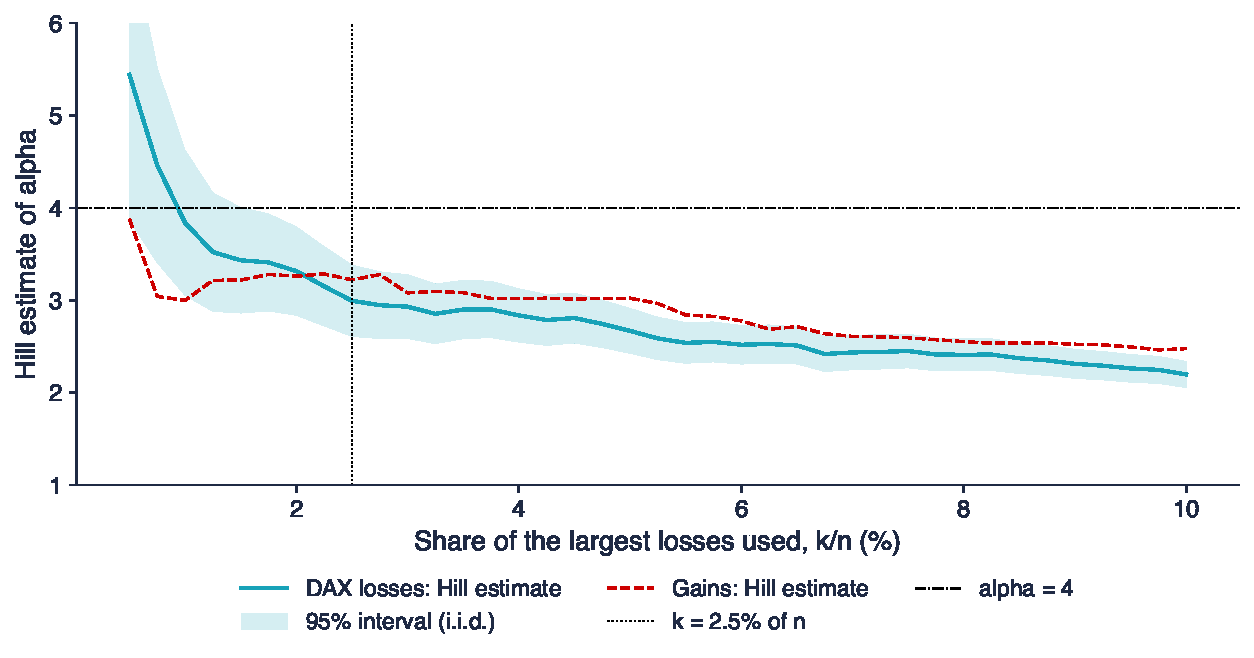
\includegraphics[width=0.96\textwidth,height=0.42\textheight,keepaspectratio]{ch5_sem_b1.pdf}
\end{center}
\vspace{-2mm}
\begin{itemize}
    \item $n = 9\,288$, $k = 232$, $L_{(k+1)} = 2{,}86\%$: $\hat\alpha = 3{,}00$, SE i.i.d.\ $0{,}20$, interval $[2{,}61; 3{,}38]$, SE blocuri $0{,}20$; cîștiguri: $3{,}22$
    \item Între $k = 1\%$ și $5\%$ din $n$, estimarea scade lent, de la $3{,}84$ la $2{,}67$; cîștigurile au o coadă mai subțire
    \item Interpretare: pentru $\alpha = 4$, statistica $z$ (cu SE pe blocuri) este $-5{,}0$: boltirea randamentelor DAX nu există, deci boltirea de selecție ($6{,}0$) nu este o mărime stabilă
\end{itemize}\quantlet{SFM\_ch5\_seminar}{\qlurl{SFM_ch5_seminar}}
\end{frame}

\begin{frame}{B2: BET, Bitcoin și două acțiuni BVB [Propus]}
\itemsize{\footnotesize}
\begin{itemize}
\item \textbf{Întrebarea}: care dintre BET, Bitcoin, OMV Petrom și Banca Transilvania are cea mai groasă coadă a pierderilor? Model: B1.
\item \textbf{Date}: BET din 1997, Bitcoin din 2014, SNP și TLV din 2010 (TLV fără 30--31 mai 2016), pierderi zilnice în \%
\item \textbf{Cerințe}
\begin{enumerate}
    \item Calculați $\hat\alpha$ la $k = 2{,}5\%$ din $n$ pentru fiecare serie, cu intervalul de 95\% și SE din bootstrap pe blocuri.
    \item Adăugați estimările la $k = 1\%$ și $5\%$ din $n$.
    \item Testați diferența dintre BET și Bitcoin cu $z = (\hat\alpha_1 - \hat\alpha_2)/\sqrt{\mathrm{SE}_1^2 + \mathrm{SE}_2^2}$.
    \item Interpretare: este coada Bitcoin mai groasă decît cea a BET, dacă lăsăm deoparte scala pierderilor?
\end{enumerate}
\item \textbf{Raportați}: un tabel, un $z$ și două fraze
\item Notebook: secțiunea B2
\end{itemize}
\end{frame}

\ifsolutions
\begin{frame}{B2: rezolvare [Propus]}
\itemsize{\footnotesize}
\begin{center}
\footnotesize
\begin{tabular}{lrrrrrr}
\toprule
& $n$ & $k$ & $\hat\alpha$ & interval 95\% & SE blocuri & $k = 1\%$ / $5\%$ \\
\midrule
BET & 7\,243 & 181 & $2{,}57$ & $[2{,}20; 2{,}95]$ & $0{,}23$ & $2{,}70$ / $2{,}16$ \\
Bitcoin & 4\,384 & 109 & $2{,}71$ & $[2{,}20; 3{,}21]$ & $0{,}23$ & $3{,}83$ / $2{,}49$ \\
OMV Petrom (SNP) & 3\,815 & 95 & $2{,}96$ & $[2{,}36; 3{,}56]$ & $0{,}39$ & $2{,}89$ / $2{,}60$ \\
Banca Transilvania (TLV) & 3\,788 & 94 & $2{,}49$ & $[1{,}98; 2{,}99]$ & $0{,}28$ & $3{,}05$ / $2{,}35$ \\
\bottomrule
\end{tabular}
\end{center}
\begin{itemize}
    \item BET față de Bitcoin: $z = -0{,}42$: nicio diferență semnificativă a indicelui de coadă
    \item Toate cele patru estimări sînt între $2{,}49$ și $2{,}96$; TLV are cel mai mic $\hat\alpha$, BET al doilea
    \item Interpretare: pierderile Bitcoin sînt mult mai mari (pragul $L_{(k+1)}$ este de două-trei ori mai mare), dar forma cozii este asemănătoare: scala și indicele de coadă sînt lucruri diferite
\end{itemize}\quantlet{SFM\_ch5\_seminar}{\qlurl{SFM_ch5_seminar}}
\end{frame}
\fi

\begin{frame}{B3: POT pentru BET [Rezolvat]}
\itemsize{\scriptsize}
\begin{itemize}
\item \textbf{Întrebarea}: cît de mari sînt VaR 1\%, ES 2,5\% și VaR 0,1\% ale pierderilor zilnice BET prin EVT, comparate cu simularea istorică și cu distribuția Normală?
\item \textbf{Date}: închiderile BET din 1997, pierderi zilnice în \%; $u$ = cuantila de 90\% a pierderilor
\item \textbf{Cerințe}
\begin{enumerate}
    \item Desenați funcția mean excess empirică și marcați $u$.
    \item Ajustați o GPD la excesele peste $u$ prin verosimilitate maximă; raportați $\hat\xi$ cu SE și $\hat\beta$.
    \item Desenați graficul QQ al exceselor față de distribuția GPD ajustată.
    \item Calculați VaR 1\%, ES 2,5\% și VaR 0,1\% prin EVT, prin simulare istorică și cu distribuția Normală.
    \item Interpretare: ce metodă ați folosi pentru capitalul unei bănci care deține BET și de ce?
\end{enumerate}
\item \textbf{Raportați}: cele două grafice, un tabel cu nouă valori și două fraze
\item Notebook: secțiunea B3
\end{itemize}
\end{frame}

\begin{frame}{B3: rezolvare [Rezolvat]}
\itemsize{\scriptsize}
\begin{center}
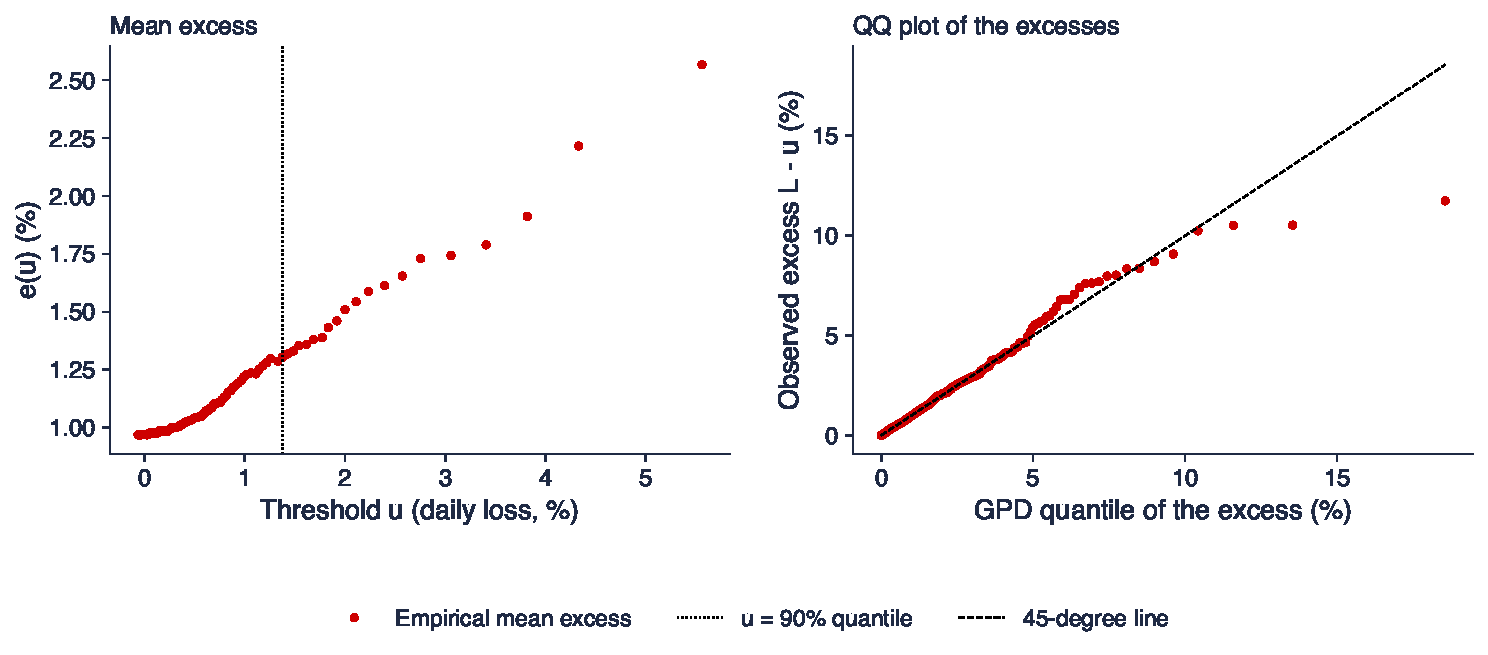
\includegraphics[width=0.96\textwidth,height=0.34\textheight,keepaspectratio]{ch5_sem_b3.pdf}
\end{center}
\vspace{-2mm}
\begin{center}
\scriptsize
\begin{tabular}{lrrr}
\toprule
(\%) & EVT & istoric & Normal \\
\midrule
VaR 1\% & $4{,}44$ & $4{,}33$ & $3{,}39$ \\
ES 2,5\% & $4{,}81$ & $4{,}80$ & $3{,}41$ \\
VaR 0,1\% & $9{,}56$ & $9{,}64$ & $4{,}52$ \\
\bottomrule
\end{tabular}
\end{center}
\begin{itemize}
    \item $n = 7\,243$, $u = 1{,}375\%$, $N_u = 725$; $\hat\xi = 0{,}223$ (SE $0{,}047$), $\hat\beta = 1{,}018$; funcția mean excess crește liniar peste $u$; punctele graficului QQ stau pe dreaptă, cu excepția celor mai mari excese
    \item Interpretare: aș folosi EVT, care concordă cu datele la 1\% și dă un VaR 0,1\% stabil; VaR 0,1\% Normal este mai mic decît jumătate din cel EVT
\end{itemize}\quantlet{SFM\_ch5\_seminar}{\qlurl{SFM_ch5_seminar}}
\end{frame}

\begin{frame}{B4: contează pragul? Bitcoin [Propus]}
\itemsize{\footnotesize}
\begin{itemize}
\item \textbf{Întrebarea}: cît de mult se schimbă $\hat\xi$ și măsurile de risc EVT pentru Bitcoin odată cu pragul? Model: B3.
\item \textbf{Date}: Bitcoin din 2014, pierderi zilnice în \%; $u$ la cuantilele de 85\%, 90\% și 95\%
\item \textbf{Cerințe}
\begin{enumerate}
    \item Pentru fiecare prag, ajustați GPD și raportați $u$, $N_u$, $\hat\xi$ cu SE și $\hat\beta$.
    \item Calculați VaR 1\%, ES 2,5\% și VaR 0,1\% pentru fiecare prag și prin simulare istorică.
    \item Interpretare: care mărime este robustă la alegerea lui $u$, $\hat\xi$ sau VaR?
\end{enumerate}
\item \textbf{Raportați}: un tabel și două fraze
\item Notebook: secțiunea B4
\end{itemize}
\end{frame}

\ifsolutions
\begin{frame}{B4: rezolvare [Propus]}
\itemsize{\footnotesize}
\begin{center}
\footnotesize
\begin{tabular}{lrrrrrrr}
\toprule
$u$ la & $u$ (\%) & $N_u$ & $\hat\xi$ (SE) & $\hat\beta$ & VaR 1\% & ES 2,5\% & VaR 0,1\% \\
\midrule
85\% & $2{,}40$ & 658 & $0{,}15$ ($0{,}04$) & $2{,}37$ & $10{,}30$ & $10{,}90$ & $20{,}06$ \\
90\% & $3{,}33$ & 439 & $0{,}12$ ($0{,}05$) & $2{,}66$ & $10{,}38$ & $10{,}90$ & $19{,}61$ \\
95\% & $5{,}33$ & 220 & $0{,}16$ ($0{,}07$) & $2{,}65$ & $10{,}23$ & $10{,}84$ & $19{,}88$ \\
istoric & & & & & $10{,}51$ & $10{,}84$ & $18{,}05$ \\
\bottomrule
\end{tabular}
\end{center}
\begin{itemize}
    \item $\hat\xi$ variază între praguri cu aproximativ o SE; măsurile de risc variază doar cu cîteva zecimi de punct procentual
    \item Interpretare: VaR și ES sînt robuste la $u$ (ajustarea modifică $\beta$); $\hat\xi$, și orice extrapolare mult dincolo de date, nu
\end{itemize}\quantlet{SFM\_ch5\_seminar}{\qlurl{SFM_ch5_seminar}}
\end{frame}
\fi

\begin{frame}{B5: maximele trimestriale ale S\&P 500 [Rezolvat]}
\itemsize{\footnotesize}
\begin{itemize}
\item \textbf{Întrebarea}: cît de mare este pierderea zilnică pe care S\&P 500 o depășește o dată la 10 ani, conform unei ajustări GEV la maximele trimestriale?
\item \textbf{Date}: închiderile S\&P 500 din 1990, cea mai mare pierdere zilnică din fiecare trimestru calendaristic
\item \textbf{Cerințe}
\begin{enumerate}
    \item Construiți maximele trimestriale ale pierderilor zilnice.
    \item Ajustați o GEV prin verosimilitate maximă; raportați $\hat\xi$ cu intervalul de 95\%, $\hat\mu$ și $\hat\sigma$.
    \item Desenați graficul QQ și graficul return levels.
    \item Calculați return level-ul de 10 ani (40 de trimestre) și numărați trimestrele în care a fost depășit.
    \item Interpretare: este coada S\&P 500 de tip Fréchet sau Gumbel?
\end{enumerate}
\item \textbf{Raportați}: trei parametri, un nivel, graficele și o frază
\item Notebook: secțiunea B5
\end{itemize}
\end{frame}

\begin{frame}{B5: rezolvare [Rezolvat]}
\itemsize{\footnotesize}
\begin{center}
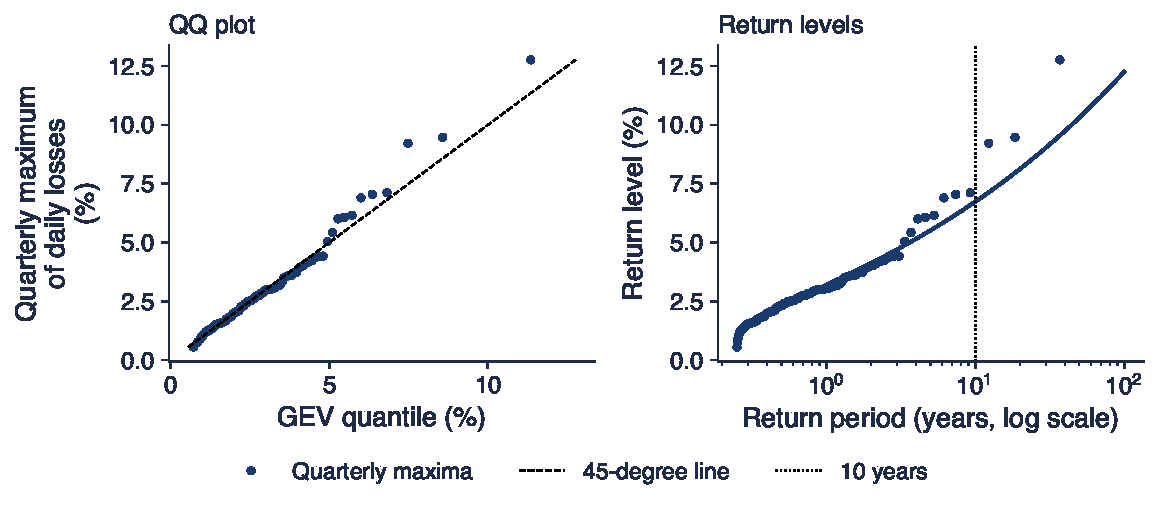
\includegraphics[width=0.96\textwidth,height=0.42\textheight,keepaspectratio]{ch5_sem_b5.pdf}
\end{center}
\vspace{-2mm}
\begin{itemize}
    \item 147 trimestre: $\hat\xi = 0{,}21$, interval de 95\% $[0{,}09; 0{,}32]$; $\hat\mu = 1{,}97\%$, $\hat\sigma = 0{,}86\%$
    \item Return level-ul de 10 ani: $6{,}7\%$; depășit în 6 din 147 trimestre ($3{,}7$ așteptate în 36{,}8 ani); cea mai mare pierdere $12{,}8\%$
    \item Interpretare: $\xi = 0$ este în afara intervalului: Fréchet, o coadă groasă cu $\alpha = 1/\hat\xi = 4{,}8$
\end{itemize}\quantlet{SFM\_ch5\_seminar}{\qlurl{SFM_ch5_seminar}}
\end{frame}

\begin{frame}{B6: rezistă VaR 1\% într-o perioadă nouă? [Propus]}
\itemsize{\footnotesize}
\begin{itemize}
\item \textbf{Întrebarea}: estimat pînă în 2014, este VaR 1\% al pierderilor DAX și BET depășit în circa 1\% din zilele din 2015--2026? Modele: B3, B5.
\item \textbf{Date}: DAX din 1990, BET din 1997, pierderi zilnice în \%; estimare pînă la 31 decembrie 2014, test după aceea
\item \textbf{Cerințe}
\begin{enumerate}
    \item Estimați VaR 1\% pe prima perioadă prin EVT (POT, $u$ la cuantila de 90\%), simulare istorică și distribuția Normală.
    \item Numărați zilele de test cu o pierdere peste fiecare VaR și comparați cu $np$.
    \item Calculați valoarea $p$ binomială bilaterală a fiecărui număr de depășiri.
    \item Interpretare: de ce pot eșua toate cele trei metode în aceeași direcție?
\end{enumerate}
\item \textbf{Raportați}: un tabel cu șase numere de depășiri și valorile $p$, plus două fraze
\item Notebook: secțiunea B6
\end{itemize}
\end{frame}

\ifsolutions
\begin{frame}{B6: rezolvare [Propus]}
\itemsize{\footnotesize}
\begin{center}
\footnotesize
\begin{tabular}{lrrrrr}
\toprule
& zile de test & așteptat & EVT (valoarea $p$) & istoric & Normal \\
\midrule
DAX & 2\,972 & $29{,}7$ & 14 ($0{,}002$) & 11 ($< 0{,}001$) & 36 ($0{,}288$) \\
BET & 2\,925 & $29{,}2$ & 8 ($< 0{,}001$) & 8 ($< 0{,}001$) & 13 ($0{,}001$) \\
\bottomrule
\end{tabular}
\end{center}
\begin{itemize}
    \item VaR 1\% (\%): DAX: EVT $4{,}12$, istoric $4{,}32$, Normal $3{,}34$; BET: $5{,}07$, $5{,}13$, $3{,}99$
    \item EVT și simularea istorică: mult mai puține depășiri decît se așteaptă (estimări prea prudente); VaR Normal trece testul pentru DAX din întîmplare: o coadă prea subțire compensată de o varianță prea mare
    \item Interpretare: perioada 2015--2026 a fost mai liniștită decît 1990--2014; un VaR necondiționat nu se adaptează regimului de volatilitate (\sfmchlink{https://danpele.github.io/SFM/RO/Cursuri/capitol9_modele_arch_garch.pdf}{Capitolele 9} și \sfmchlink{https://danpele.github.io/SFM/RO/Cursuri/capitol10_var_es_backtesting.pdf}{10})
\end{itemize}\quantlet{SFM\_ch5\_seminar}{\qlurl{SFM_ch5_seminar}}
\end{frame}
\fi


%=============================================================================
\section{Partea C: întrebări deschise și critica unui răspuns AI}
%=============================================================================

\begin{frame}{C1: s-a schimbat coada Bitcoin? [Propus]}
\itemsize{\footnotesize}
\begin{itemize}
\item \textbf{Întrebarea}: este indicele de coadă al pierderilor Bitcoin diferit în 2014--2017, 2018--2021 și 2022--2026?
\item \textbf{Date}: pierderile zilnice Bitcoin din 2014, împărțite în trei perioade; modele: B1, B2
\item \textbf{Cerințe}
\begin{enumerate}
    \item Calculați $\hat\alpha$ Hill la $k = 2{,}5\%$ din $n$ în fiecare perioadă, cu SE din bootstrap pe blocuri și un interval de 95\%.
    \item Stabiliți dacă vreo pereche de perioade diferă semnificativ.
    \item Propuneți o schimbare a metodei care ar da un răspuns mai clar.
    \item Interpretare: ce poate spune un eșantion de circa 1\,500 de zile despre un indice de coadă?
\end{enumerate}
\item \textbf{Raportați}: un tabel, o frază pentru fiecare comparație și un plan de proiect
\item Notebook: secțiunea C1
\end{itemize}
\end{frame}

\ifsolutions
\begin{frame}{C1: analiză de referință [Propus]}
\itemsize{\footnotesize}
\begin{center}
\footnotesize
\begin{tabular}{lrrrrr}
\toprule
Perioada & $n$ & $k$ & $\hat\alpha$ & SE blocuri & interval 95\% \\
\midrule
2014--2017 & 1201 & 30 & $2{,}68$ & $0{,}45$ & $[1{,}79; 3{,}57]$ \\
2018--2021 & 1461 & 36 & $3{,}23$ & $0{,}71$ & $[1{,}85; 4{,}62]$ \\
2022--2026 & 1722 & 43 & $2{,}88$ & $0{,}43$ & $[2{,}03; 3{,}74]$ \\
\bottomrule
\end{tabular}
\end{center}
\begin{itemize}
    \item Toate intervalele se suprapun: nicio schimbare semnificativă; cu $k$ între 30 și 43, SE este $0{,}43$--$0{,}71$
    \item Variante mai clare: pierderi standardizate cu GARCH (\sfmchlink{https://danpele.github.io/SFM/RO/Cursuri/capitol9_modele_arch_garch.pdf}{Capitolul 9}), POT cu un prag comun, mai multe active cripto împreună, ferestre mai lungi
    \item Interpretare: circa 1\,500 de zile oferă circa 40 de observații în coadă: suficient pentru un $\alpha$ aproximativ, nu pentru a detecta o schimbare de 0,5
\end{itemize}\quantlet{SFM\_ch5\_seminar}{\qlurl{SFM_ch5_seminar}}
\end{frame}
\fi

\begin{frame}{C2: verificați un răspuns AI [Propus]}
\itemsize{\scriptsize}
\begin{itemize}
    \item Un student a cerut unui asistent AI să estimeze coada pierderilor zilnice S\&P 500 din 1990 prin POT. Răspunsul:
    \item \aiprompt{(a) Cu u = 1{,}163\%, N\_u = 924 din n = 9\,240, GPD dă xi = 0{,}158, deci indicele de coadă este alpha = 0{,}158, iar varianța este infinită.}
    \item \aiprompt{(b) VaR 1\% = u + (beta/xi) [(n p / N\_u)\textasciicircum xi - 1] = -0{,}32\%.}
    \item \aiprompt{(c) ES 2,5\% = VaR 2,5\% x (1 - xi) = 1{,}98\%.}
    \item \aiprompt{(d) Aceeași formulă dă un VaR 20\% fiabil.}
    \item \aiprompt{(e) Peste u, funcția mean excess a GPD ajustate este o dreaptă în funcție de prag.}
    \item Cerințe
    \begin{itemize}
        \item 1. Pentru fiecare afirmație stabiliți dacă este corectă; dacă nu este, formulați afirmația corectă și, unde se poate, dați valoarea corectă din notebook (secțiunea C2).
        \item 2. Raportați: o listă de cinci verdicte, fiecare cu un rînd de justificare.
    \end{itemize}
\end{itemize}
\end{frame}

\ifsolutions
\begin{frame}{C2: rezolvare [Propus]}
\itemsize{\footnotesize}
\begin{itemize}
    \item (a) Greșit: $\alpha = 1/\xi = 6{,}3$, nu $\xi$; varianța unei cozi GPD este finită pentru $\xi < 1/2$
    \item (b) Greșit: exponentul este $-\xi$; VaR 1\% $= 3{,}30\%$ (un VaR negativ, $-0{,}32\%$, sub $u$, este un semnal de alarmă)
    \item (c) Greșit: $\mathrm{ES}_p = (\mathrm{VaR}_p + \beta - \xi u)/(1 - \xi)$: VaR 2,5\% $= 2{,}35\%$, ES 2,5\% $= 3{,}49\%$; ES nu poate fi niciodată sub VaR
    \item (d) Greșit: GPD modelează doar cele mai mari $N_u/n = 10\%$ dintre pierderi; este valabilă doar pentru $p < 10\%$
    \item (e) Corect: $e(v) = (\beta + \xi(v - u))/(1 - \xi)$ pentru $v > u$, liniară, cu panta $\xi/(1 - \xi)$
\end{itemize}\quantlet{SFM\_ch5\_seminar}{\qlurl{SFM_ch5_seminar}}
\end{frame}
\fi


%=============================================================================
\section{Încheiere}
%=============================================================================

\begin{frame}{Idei de reținut}
\itemsize{\small}
\begin{itemize}
    \item Pierderile zilnice au cozi de tip putere cu $\alpha$ între 2,5 și 3,5: varianță finită, boltire infinită
    \item Hill: fixați $k$ într-o zonă plată a graficului Hill; raportați o eroare standard care ține seama de volatility clustering
    \item POT: $u$ la o cuantilă înaltă, GPD pentru excese, VaR și ES prin formule explicite; verificați cu mean excess și grafice QQ
    \item Block maxima: GEV, Fréchet pentru pierderile financiare; return levels dincolo de eșantion sînt extrapolare
    \item Un răspuns AI este o ciornă: verificați $\alpha = 1/\xi$, semnul exponentului, ES $\ge$ VaR și domeniul $p < N_u/n$
\end{itemize}
\end{frame}

\begin{frame}{După seminar}
\itemsize{\small}
\begin{itemize}
    \item Cursul 5 dezvoltă fiecare temă de azi: crahuri, variație regulată, Hill, mean excess, GEV, GPD, VaR și ES prin EVT
    \item Încercați cerințele [Propus] în notebook; rezolvările se discută la seminar
    \item C1 poate deveni un proiect de echipă: pierderi standardizate cu GARCH, POT cu prag comun, mai multe active cripto
    \item Lectură: \refFHH, cap.~18; exerciții în \refBHL, cap.~18; \refQRM, cap.~5
\end{itemize}
\end{frame}


%=============================================================================
\section{Bibliografie}
%=============================================================================

\begin{frame}{Bibliografie}
\itemsize{\tiny}
\begin{itemize}
    \item Balkema, A.A., de Haan, L. (1974). \href{https://doi.org/10.1214/aop/1176996548}{Residual life time at great age}. \textit{Annals of Probability}, 2(5), 792--804.
    \item Borak, S., Härdle, W.K., López-Cabrera, B. (2013). \href{https://doi.org/10.1007/978-3-642-33929-5}{\textit{Statistics of Financial Markets: Exercises and Solutions}}, 2nd ed. Springer.
    \item Fisher, R.A., Tippett, L.H.C. (1928). \href{https://doi.org/10.1017/S0305004100015681}{Limiting forms of the frequency distribution of the largest or smallest member of a sample}. \textit{Mathematical Proceedings of the Cambridge Philosophical Society}, 24(2), 180--190.
    \item Franke, J., Härdle, W.K., Hafner, C.M. (2019). \href{https://doi.org/10.1007/978-3-030-13751-9}{\textit{Statistics of Financial Markets: An Introduction}}, 5th ed. Springer.
    \item Gnedenko, B. (1943). \href{https://doi.org/10.2307/1968974}{Sur la distribution limite du terme maximum d'une série aléatoire}. \textit{Annals of Mathematics}, 44(3), 423--453.
    \item Hill, B.M. (1975). \href{https://doi.org/10.1214/aos/1176343247}{A simple general approach to inference about the tail of a distribution}. \textit{Annals of Statistics}, 3(5), 1163--1174.
    \item McNeil, A.J., Frey, R. (2000). \href{https://doi.org/10.1016/S0927-5398(00)00012-8}{Estimation of tail-related risk measures for heteroscedastic financial time series: an extreme value approach}. \textit{Journal of Empirical Finance}, 7(3--4), 271--300.
    \item McNeil, A.J., Frey, R., Embrechts, P. (2015). \href{https://press.princeton.edu/books/hardcover/9780691166278/quantitative-risk-management}{\textit{Quantitative Risk Management: Concepts, Techniques and Tools}}, revised ed. Princeton University Press.
    \item Pickands, J. (1975). \href{https://doi.org/10.1214/aos/1176343003}{Statistical inference using extreme order statistics}. \textit{Annals of Statistics}, 3(1), 119--131.
    \item Weissman, I. (1978). \href{https://doi.org/10.1080/01621459.1978.10480104}{Estimation of parameters and large quantiles based on the $k$ largest observations}. \textit{Journal of the American Statistical Association}, 73(364), 812--815.
\end{itemize}
\end{frame}

\end{document}
